%\section{Photon Detection System (PDS) Overview}
%%%%%%%%%%%%%%%%%%%%%%%%%%%%%%%%%%%%%%%%%%%%%%%%%%%%
\section{Introduction} % Anne
\label{sec:fdsp-pd-intro}
%\metainfo{\color{blue} Content: Segreto, Warner, Wilson}

%\metainfo{(Length: \dword{tdr}=10 pages, TP=3 pages)}
%Tim drafted some potential text to begin with: (anne)
%rjw 1/9/19 minor changes.

The DUNE \dword{fd} consists of detector systems for charge and light produced by an ionization event in the \lartpc.  The charge detection system permits both calorimetry and position determination, with two of the three spatial coordinates ($y$ and $z$)  established by the position of the \dword{apa} wires receiving the charge and the third ($x$) by the arrival time of the charge.  Locating the $x$ position requires an independent determination of the time of the ionization event, a clock start time.  Two systems provide this in DUNE:  the Fermilab accelerator system for neutrino beam related events and the \dword{pds}.  

Neutrino \dword{cpv} and other elements of the DUNE long-baseline neutrino program do not rely, to first order, on the \dword{pds}.  The neutrino beam timing allows full functionality of the \dword{apa}s, and the deep underground location reduces the possibility of in-time background events from cosmic rays and other sources to a negligible level.  
Similarly, DUNE can detect \dwords{snb} originating within the galaxy without a \dword{pds}.  In this case, the presence of thousands of even very low energy (\SI{5}-\SI{30}{MeV}) events, consisting of tracks only a few millimeters long, occurring over tens of seconds would provide an unambiguous signal that the TPC could characterize on its own.
By contrast, DUNE's nucleon decay physics could not be executed without the \dword{pds}.  The inability to establish a clock start time would make it impossible to determine whether a candidate proton decay event was fully contained in the detector volume or associated with objects entering the detector from the outside.  

While only absolutely required for proton decay searches, the \dword{pds} directly enhances physics capabilities for all three DUNE physics drivers, opens up prospects for further physics explorations, and contributes to a more robust set of operating points of the detector that help all physics.   For beam neutrino physics, for example, the \dword{pds} improves the ability to pick up the relatively late time Michel electron produced from the decay of a stopped muon.  In addition to providing a useful calibration source for low energy electrons,  this aids an in situ statistical determination of the antineutrino content of the beam. While 75\% of $\mu^-$ are captured by the nucleus before they decay, all $\mu^+$ produce a Michel electron.  Michel electron tagging assists in background suppression for similar reasons in proton decay searches.  The $p\rightarrow K^+\nu$ mode produces a distinct $K^+\rightarrow\mu^+\rightarrow e^+$ topology.  Picking up the Michel electron at the end of the sequence can help suppress topologically and calorimetrically similar signals from atmospheric neutrino induced $\mu^- p$ final states.  

For \dword{snb} neutrino events, the \dword{pds} allows for proper location of the event vertex and the implementation of position-dependent corrections for charge loss due to electron capture and other transport effects in the TPC, leading to improved energy resolution and possibly greater sensitivity to underlying supernova dynamical models.  The \dword{pds} could open new areas of investigation.  The few-MeV scale solar neutrino interactions occur as isolated events in time and space.  Suppression of radiological and noise related backgrounds to pull out a signal for these events likely requires  redundant measurements with charge and light.  In the event that the DUNE TPC could not operate at its goal electric field of \SI{500}{V/cm}, the \dword{pds} can compensate for lessened charge detector performance:  Light production increases relative to that of free charge for lower \efield{}, and calorimetry using this light production offers a chance of maintaining the overall resolution of the detector. For \dword{snb} physics, the \dword{pds} enables a triggering scheme that greatly assists the \dword{daq} system in maintaining minimal dead time.
 
%The remaining sections further develop the specification and design of a \dword{pds} that supports DUNE physics.

The Physics TDR (Vol.~2) describes the detailed physics simulations of the main DUNE physics drivers.  In the following section we describe additional simulations performed to establish the \dword{pds} performance specifications that are met or exceeded by the design described in the rest of this chapter.
 


% Anne took this part out 12/27: The \dword{pds} is an essential detector subsystem of a DUNE \dword{spmod}. The detection of the prompt scintillation light signal, emitted in coincidence with an ionizing event inside the active volume, allows the determination of the time of occurrence of an event of interest with much higher precision than charge collected from ionization in the TPC. This capability is most critical for the primary DUNE science objectives that are uncorrelated with the timing signal from the neutrino source at \fnal, such as proton decay and neutrinos from a \dword{snb}, and for the ancillary science program including measurements of neutrino oscillation phenomena using atmospheric neutrinos. 



% Anne took this part out 12/27: Timing information from the \dword{pd} and TPC systems allows determination of the drift time of the ionizing particles. Knowledge of the drift time provides localization of the event inside the active volume and %provides the ability to enables corrections to the measured charge for effects that depend on the drift path length, purity of \lar, or for specific locations in the detector %if there are due to non-uniformities.  This correction is important for %the reconstruction of the energy deposited by the ionizing event. In addition to allowing optimum track reconstruction, scintillation light measured by the system may also be used as a trigger and for improved calorimetric measurement in combination with charge measurement.

%%%%%%%%%%%%%%%%%%%%%%%%%%%%%%%%%%%%%%%%%%%%%%%%%%%%%%%%%%%%%%%%%%%%%%%%%%%%%%%%
%rjw 1/9/19 Try Simulation as part of the introduction 
%%%%%%%%%%%%%%%%%%%%%%%%%%%%%%%%%%%%%%%%%%%%%%%%%%%%%%%%%%%%%%%
%
\subsection{Simulation}
\label{sec:fdsp-pd-simphys}
% Provided by Alex H. 15mar18
%\metainfo{Content: Himmel}


The broad performance specifications for the \dword{pds} are determined by a series of physics deliverables addressing the major physics goals of DUNE: nucleon decay searches, supernova burst neutrinos, and beam neutrinos. Detailed sub-detector specifications, such as light yield of the light collectors, are determined using a full simulation, reconstruction, and analysis chain developed for the \larsoft framework. 

\subsubsection{Simulation and Reconstruction Steps} 
\label{subsec:fdsp-pd-simphys-sim}

The first step in the simulation specific to the \dword{pds} is the simulation of the production of light and its transport within the volume to the \dwords{pd}. Argon is a strong scintillator, producing \SI{24000}{$\gamma$s/MeV} at our nominal drift field. Even accounting for the efficiency of the \dwords{pd}, it is prohibitive to simulate every optical photon with \dword{geant4} in every event. So, prior to the full event simulation, the detector volume is voxelized and many photons are produced in each voxel. The fraction of photons from each voxel reaching each photosensor is called the visibility, and these visibilities are recorded in a 4-dimensional library.
This library includes Rayleigh scattering length ($\lambda_R=$ \SI{60}{cm}~\cite{Grace:2015yta}), absorption length ($\lambda_A=$ \SI{20}{m}), and the measured collection efficiency versus position of the double-shift light-guide bars. There is significant uncertainty on the scattering length in the literature, so the value is conservatively chosen at the low end of those reported. With these optical properties, there is a factor of 20 difference in total amount of light collected between events right in front of the photon detectors and those on the far side of the drift volume \SI{3.6}{m} away. 

%When a particle is simulated, at each step it produces charge and light. The light produced 
When a particle trajectory is simulated, the amount of charge and light it produces is calculated in small steps. The light produced in each step is 
distributed onto the various \dwords{pd} using the photon library as a look-up table, and the 30\% early (\SI{6}{ns}) plus 70\% late (\SI{1.5}{$\mu$s}) scintillation time constants are applied. Transport time of the light through the \lar is not currently simulated but is under development. It is not expected to make a significant difference in the studies presented here.

The second step is the simulation of the sensor and electronics response. For the studies shown here, the SensL \dword{sipm} and \dword{sipm} signal processor (\dword{ssp}) readout electronics used for \dword{pd} development and in \dword{pdsp} is assumed (see Section~\ref{sec:fdsp-pd-pde}). However, a range of \dword{s/n} and dark rates are considered in order to set requirements on the needed performance of the electronics.
Crosstalk (where a second cell avalanches when a neighbor is struck by a photon generated internal to the silicon) is introduced by adding a second \phel \num{16.5}\% of the time when an initial \phel is added to the waveform. Additional uncorrelated random noise is added to the waveform with an RMS of
\SI{0.1}{\phel{}}. The response of the \dword{ssp} self-triggering algorithm, based on a leading-edge discriminator, is then simulated to determine if and when a \SI{7.8}{$\mu$s} waveform will be read out, or in the case of the simulation, 
stored and passed on for later processing.

The third step is reconstruction, which proceeds in three stages. The first is a ``hit finding'' algorithm that searches for peaks on individual waveforms channel-by-channel, identifying the time (based on the time of the first peak) and the total amount of light collected (based on the integral until the hit goes back below threshold). The second step is a ``flash finding'' algorithm that searches for coincident hits across multiple channels. All the coincident light is collected into a single object that has an associated time (the earliest hit), an amount of light (summed from all the hits), and a position on the plane of the \dword{apa} ($y$-$z$) that is a weighted average of the positions of the photon collectors with hits in the flash.  
The final step is to ``match'' the flash to the original event by taking the largest flash within the allowed drift time that is within \SI{240}{cm} in the $y$-$z$ plane. Since the TPC reconstruction is still in active development, especially for low-energy events, we match to the true event %\dword{mc} 
vertex of the event in the analyses presented here. This is a reasonable approximation since the position resolution of the TPC will be significantly better than that of the \dword{pds}. 

These tools (or subsets of them) are then used to evaluate how the performance of the \dword{pds} affects the following set of physics deliverables.

\subsubsection{Nucleon Decay}
\label{subsec:fdsp-pd-simphys-ndk}

Nucleon decays are rare events, so excluding backgrounds is of the utmost importance. Since some backgrounds can be generated by cosmic rays passing outside the active detector area, setting a fiducial volume to exclude such events is critically important.

\textit{Fiducialization with \tzero}\nopagebreak

The physics deliverable: the \dwords{pd} must be able to determine \tzero with approximately \SI{1}{\micro s} resolution (SP-FD-4: time resolution) for events with visible energy greater than \SI{200}{MeV} throughout the active volume and do so with $>99\%$ efficiency (SP-FD-3: light yield), as described in \physchndk{}, Section~6.1.4. 
This energy regime is relevant for nucleon decay and atmospheric neutrinos. The time measurement is needed for event localization for optimal energy resolution and rejection of entering backgrounds. 
This resolution is required for comparable spatial resolution to the TPC along the drift direction.

\begin{dunetable}[PD system efficiency for nucleon decay events]
{ccc}
{tab:pds-ndk}
{Efficiency for tagging nucleon decay events with the \dword{pds} at the \dword{cpa}, the dimmest region of the detector, which is \SI{3.6}{m} from the \dwords{pd}, shown for range of light yields (LY) at that position. Also shown is the total PD module collection efficiency required for that light yield with the simulated scattering length, \SI{60}{cm}.)}
\dword{cpa} Light yield (PE/MeV) & Collection Efficiency  (\%) & Efficiency at the \dword{cpa} (\%) \\
%(PE/MeV) & (\%) & (\%) \\ 
\toprowrule
0.09 & 0.24   & $93.8 \pm 0.4$ \\ \colhline
0.28 & 0.75  & $97.7 \pm 0.4$ \\ \colhline
0.33 & 0.88  & $98.4 \pm 0.2$ \\ \colhline
0.50 & 1.3  & $98.9 \pm 0.2$ \\ 
\end{dunetable}


The physics here feeds down to a requirement on the minimum light yield (SP-FD-3: light yield), determined by measuring how often the correct flash was not assigned to nucleon decay 
events\footnote{The most relevant sample is actually the \textit{background} to nucleon decay events. However, efficiently simulating background that can mimic nucleon decays is challenging since they can be quite rare topologies. It is therefore easier to simulate the nucleon decay signal that should be representative of the background.} 
in the dimmest region of the detector, near the \dword{cpa}. A minimum light yield of \SI{0.5}{PE/MeV} is required to meet the requirement of 99\% efficiency, as shown in Table~\ref{tab:pds-ndk}. 

A light collector with 1.3\% collection efficiency (defined as the probability that a photon reaching the surface of the light collector will be recorded as a \phel) achieves this light yield with the simulated \SI{60}{cm} scattering length. This efficiency is equivalent to having \SI{23}{cm^2} of active area per module with 100\% efficiency. At this scattering length, there is a factor of 20 difference in light yield between the brightest and dimmest regions of the detector, so techniques to improve light yield uniformity (discussed in Appendix~\ref{sec:fdsp-pd-enh}) would reduce the inefficiency still further and ease understanding the detector systematic uncertainties.


\subsubsection{Supernova Neutrinos}
\label{subsec:fdsp-pd-simphys-snb}

Supernova bursts are also rare events, though here the event is made up of many interactions (spread over several seconds) instead of a single interaction. For distant supernovae (at the far side of the Milky Way or in the Large Magellanic Cloud), the top priority is to ensure that the detector can identify a burst when it happens and trigger the detector readout. For nearby supernovae, triggering will not be a challenge, and instead the goal is to record as much information as possible about the burst.

\textit{Burst Triggering}\nopagebreak

The physics deliverable: the \dword{pds} must be able to trigger on \dwords{snb} which produce 50 neutrino interactions in a \SI{10}{kt} volume\footnote{About the amount expected for a burst at the far side of our galaxy.} with almost 100\% efficiency with a false positive rate of less than one per month. This deliverable is most important for distant supernovae where the most important requirement is that we trigger and record the data. If both the \dword{pds} and TPC triggers have good efficiency, they can provide redundancy against one another or be combined to increase efficiency or lower the background rate. The once-per-month false positive rate is determined by limits in data handling.

The \dword{pds} trigger performance was studied for a plausible but challenging signal: a supernova burst in the Large Magellanic Cloud, which we conservatively assumed would produce only 10 signal events in the far detector. The trigger efficiency was studied with variations in light yield, dark rate, and signal-to-noise ratio, keeping the requirement from the DAQ that the fake rate be held to less than one per month. The burst trigger efficiency for 10 supernova neutrino events in one \SI{10}{kt} module (a  pessimistic prediction for a supernova in the LMC), was found to be approximately $80\%$, and it is relatively insensitive to all these parameters for average light yield $>$\SI{7}{PE/MeV} (equivalent to 0.9\% collection efficiency with the simulated optical properties), dark rate $<$\SI{1}{kHz}, and signal-to-noise $>3$. The uncorrelated noise from dark rate and low signal-to-noise was easily excluded from trigger primitives by the clustering scheme, and the increased light yield makes both backgrounds and signal brighter together, so performance stays basically constant. Thus this physics deliverable, while important, does not constrain any detector requirements.


\textit{TPC Energy Measurement and Time Resolution with \tzero}\nopagebreak

The physics deliverable: the \dwords{pd} must be able to provide \tzero determination with \SI{1}{\micro s} resolution (SP-FD-4: time resolution) for at least 60\% of the neutrinos in a typical \dword{snb} energy spectrum. The \tzero measurements are used in concert with the TPC-reconstructed event in two ways: to correct for the attenuation of the charge signal as a function of how far the charge drifts through the TPC and to provide more precise absolute event times for resolving short time features in the \dword{snb} neutrino event rate. This deliverable is important primarily for nearby supernovae where the number of events is large enough that time and energy resolution will be the limiting factors in extracting physics, as described in \physchsnb{}. 

\begin{dunefigure}[Supernova neutrino energy resolution from the TPC]
{fig:pds-snb-driftcor}
{The energy resolution for supernova neutrino events when reconstructed by the TPC with the drift distance corrected using three assumptions on the performance of the \dword{pds}. The options considered range from drift correction for no events (black), to 60\% of events (blue), to 100\% of events (red).
}
  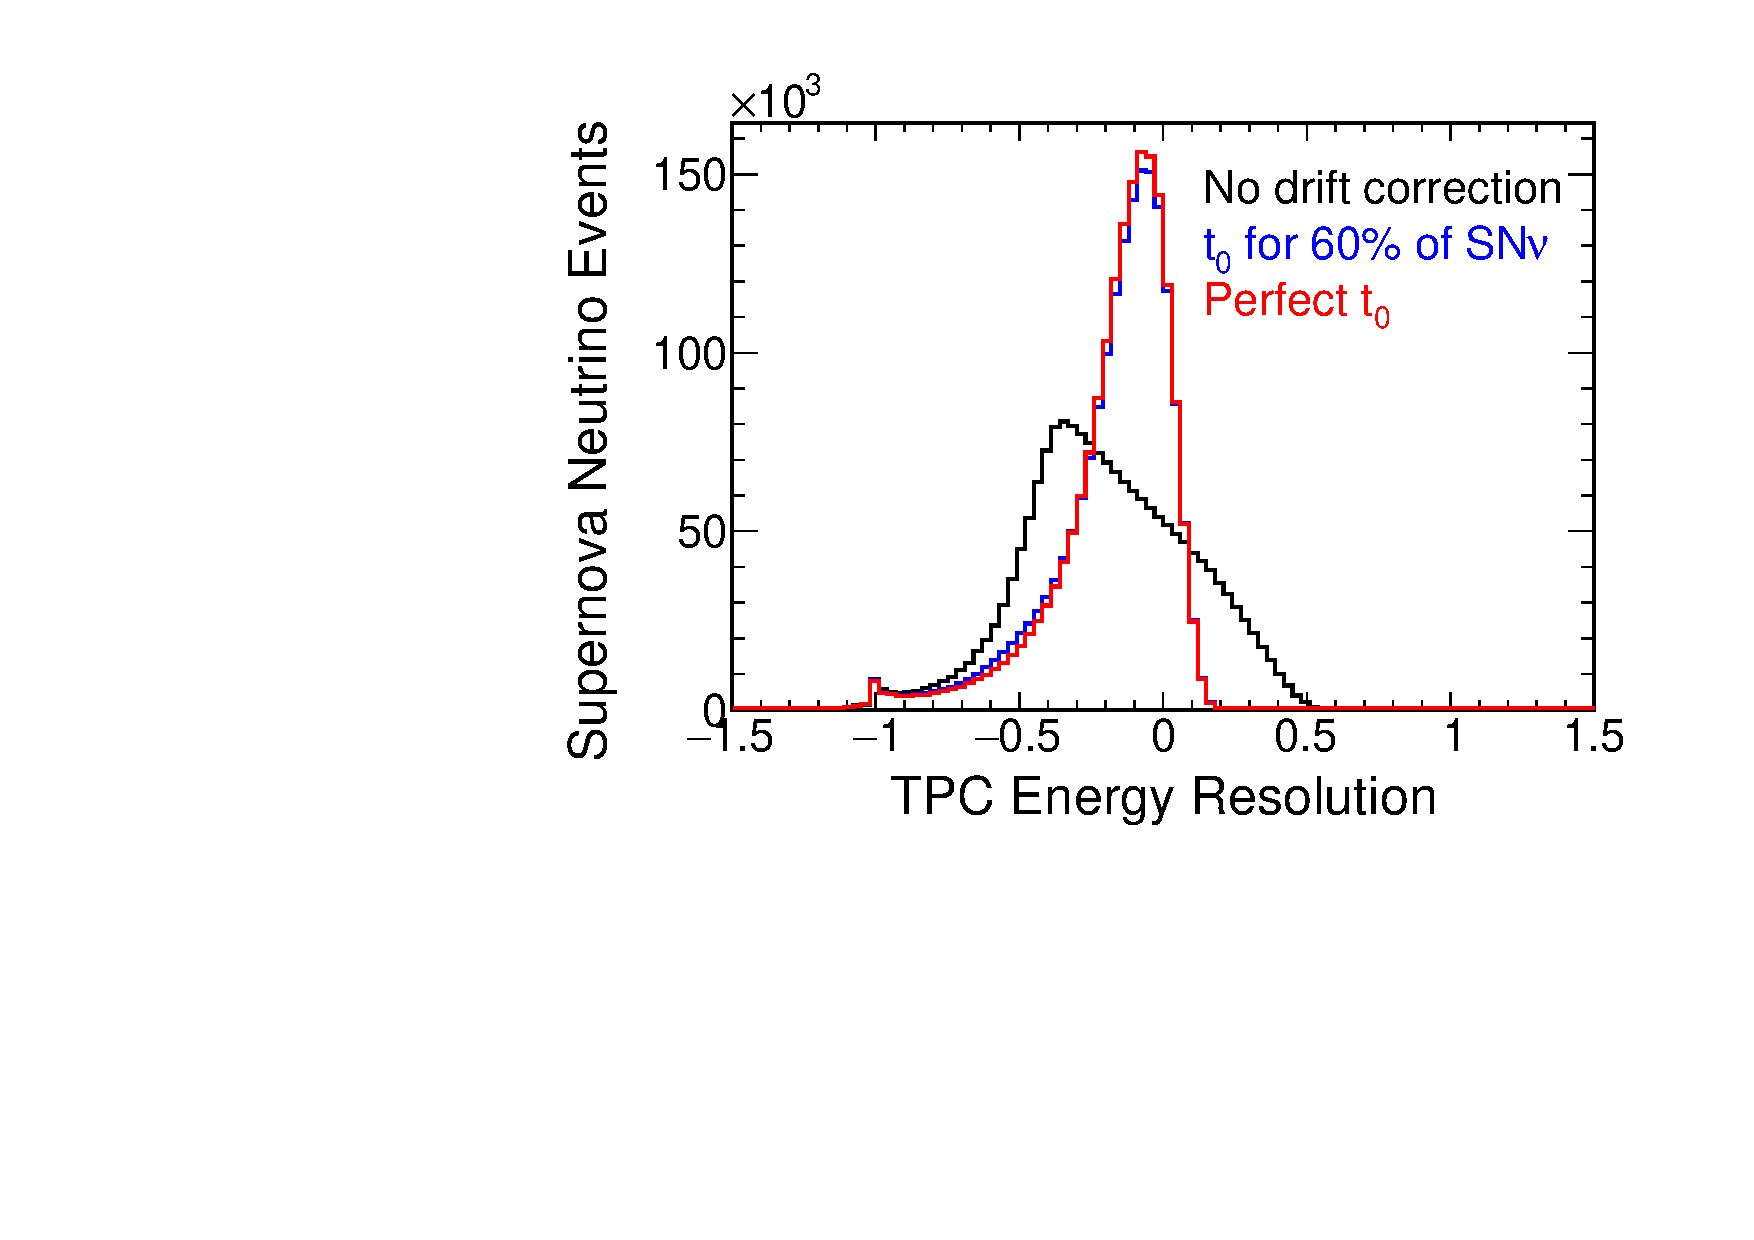
\includegraphics[width=0.5\textwidth]{graphics/pds-snb-drift-corr}
 \end{dunefigure}

The 60\% \tzero tagging requirement comes from two studies of a typical \dword{snb} neutrino spectrum under varying \dword{pd} performance assumptions: the resolution of the energy reconstructed with the TPC and drift-corrected using the time from the \dwords{pd}, and the observability of the in-fall `notch' in the \dword{snb} event time distribution. Both studies show significant improvement when going from no \dwords{pd} to a system that has a collection efficiency of at least 0.25\% (equivalent to \SI{0.5}{PE/MeV} for 60\% of the detector volume), but only marginal improvements past that point, as can be seen in Figure~\ref{fig:pds-snb-driftcor}. The light yield required here is sufficiently low that this deliverable does not set any additional detector requirements.


\textit{Calorimetric Energy}\nopagebreak

Physics deliverable: the \dword{pds} should be able to provide a calorimetric energy measurement for low-energy events, like \dwords{snb}, complementary to the TPC energy measurement. 
Improving the energy resolution will enable us to extract the maximum physics from a \dword{snb} (see \physchsnb{}), and with the goal to achieve energy resolution comparable to the TPC, we can take full advantage of the anti-correlation between the emission of light and charge signals imposed by the conservation of energy. In addition, this requirement allows the photon detection system to provide redundancy if a supernova occurs during adverse detector conditions. If the argon purification system is offline, the photon signal is significantly less sensitive to electronegative impurities, and if the drift field is low, the reduced charge signal can be partially recovered by increased light.


\begin{dunefigure}[SNB neutrino energy resolution from the PD system]
{fig:pds-snb-calo}
{The energy resolution (determined from the distribution widths of the fraction of difference between reconstructed and true to true neutrino energy for simulated events) for supernova neutrino events when reconstructed directly through \dword{pds} calorimetry for a range of light yields, represented by different colors. The red line labeled \textit{Physics} 
shows the energy smearing inherent to the neutrino interactions and thus serves as a theoretical minimum resolution. The black line shows the energy resolution achieved by the \dword{tpc}, defined in a similar way. The performance improves significantly up until approximately \SI{20}{PE/MeV} where the \dword{pds} and \dword{tpc} give comparable resolution below approximately \SI{7}{MeV}.. 
}
  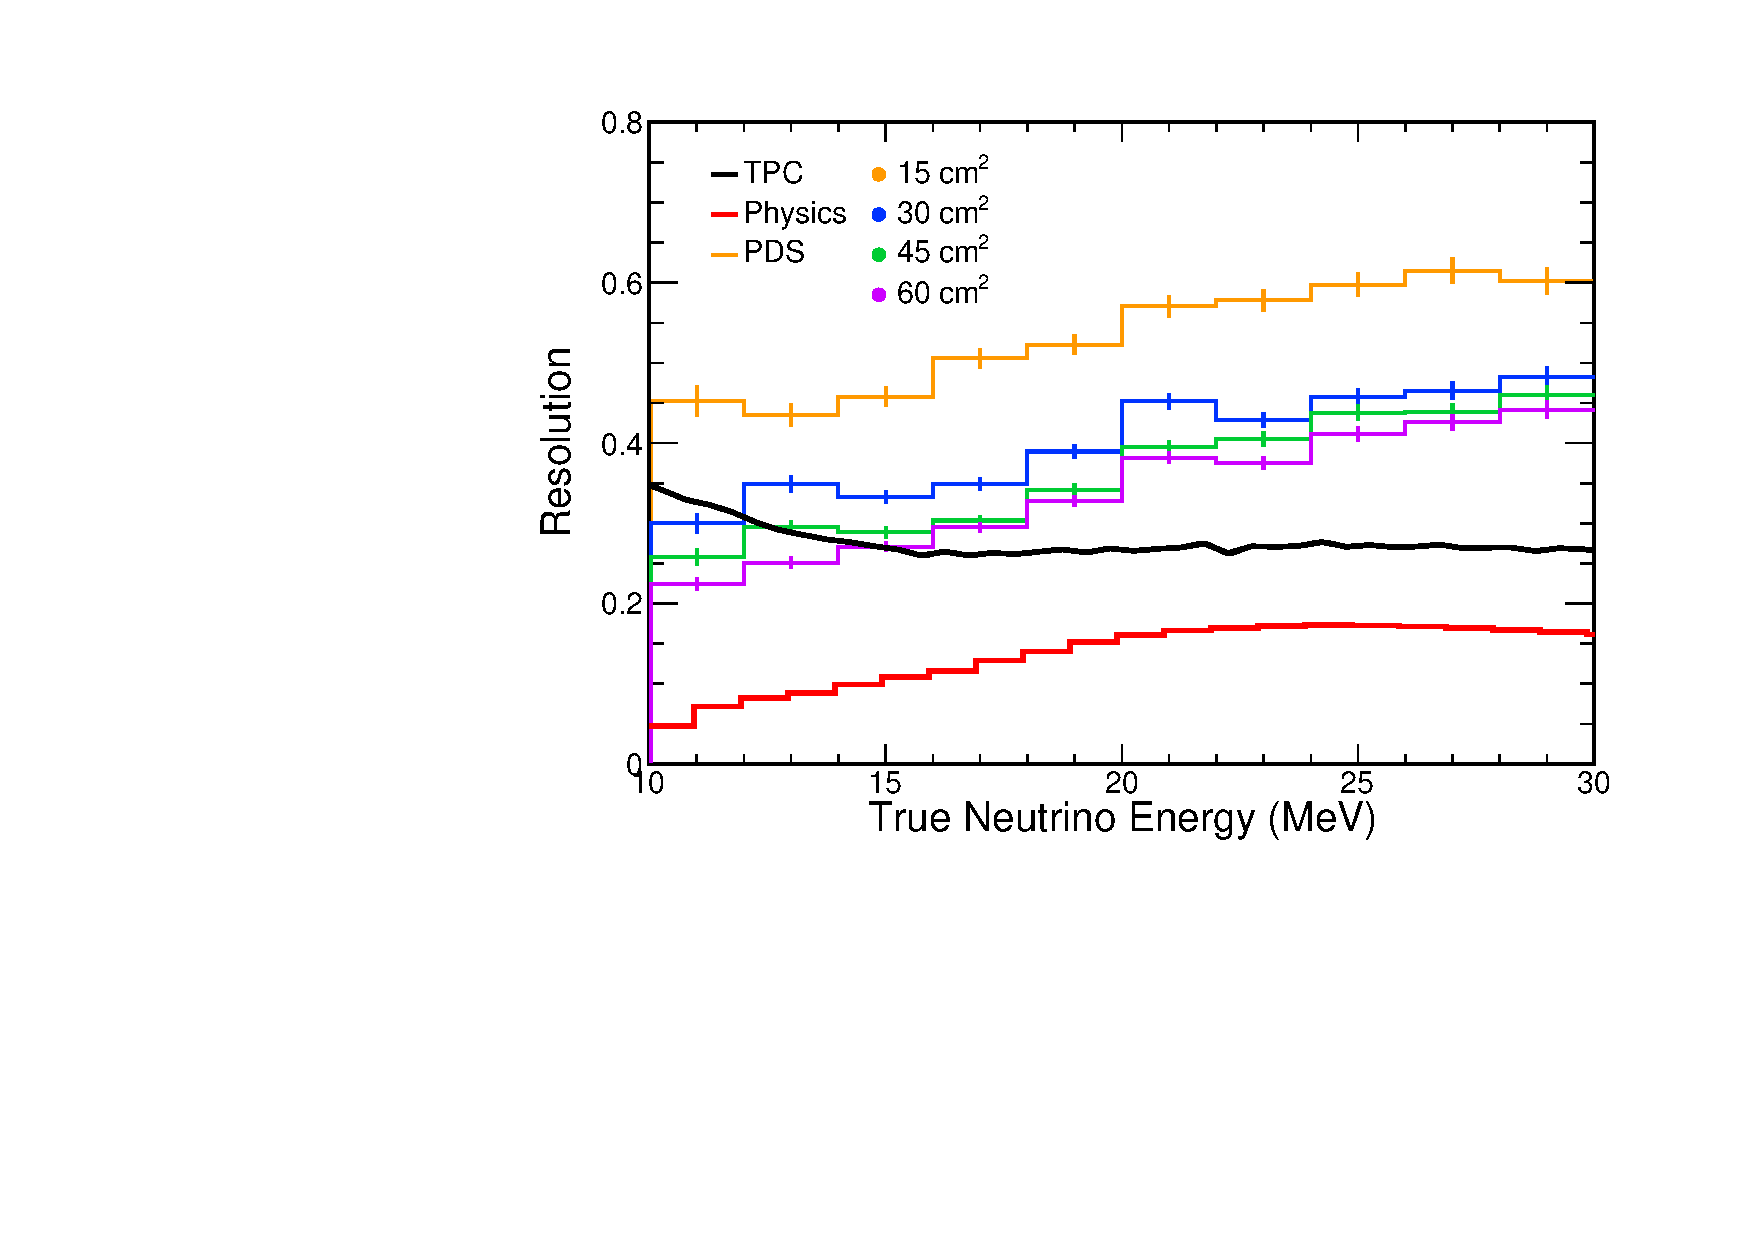
\includegraphics[width=0.6\columnwidth]{graphics/pds-snb-res-vs-true.pdf}
 \end{dunefigure}

The calorimetric energy performance was studied for supernova burst neutrino events simulated in the far detector for a range of different detector performance assumptions. The energy reconstruction was simple, correcting the total observed amount of photons for the average number of photons expected per MeV as a function of position along the drift direction. Events were required to be well away from the side walls to avoid any possible edge effects. The energy resolution vs. true energy is shown in Figure~\ref{fig:pds-snb-calo}. There is a significant benefit to achieving a photon detector with an average light yield of \SI{20}{PE/MeV}, where the \dword{pds} and \dword{tpc} have comparable resolution for the lowest energy ($<$\SI{7}{MeV}) supernova neutrinos. Past this light yield, the improvement appears to plateau in this analysis. This physics deliverable thus sets a requirement, FD-SP-3: light yield, of \SI{20}{PE/MeV} averaged over the active volume.

While options that can improve the uniformity of the detector are not essential to achieve required resolution, they are likely to improve the calorimetric energy reconstruction above and beyond total light yield. A detector that is more uniform will be easier to calibrate, and the impact of uncertainties on the optical parameters of the liquid argon will be reduced. This effect is potentially important for supernova neutrinos, and certainly more important for the beam neutrino events described in the next section. In addition, for Xe-doping specifically, speeding up the late light will allow for flashes that are narrower in time, reducing the amount of radiological contamination mixed in with the signal, which is of particular importance with these relatively small signals.


\subsubsection{Beam Neutrinos}
\label{subsec:fdsp-pd-simphys-beam}

The \dword{pds} is not required for fiducializing beam neutrino events since the pulsed beam will provide sufficient precision to place the interactions in space. However, the \dwords{pd} can potentially contribute to the energy measurement, and the better timing resolution can help identify Michel electrons from muon and pion decay.


\textit{Calorimetric Energy}\nopagebreak

Physics deliverable: the \dword{pds} should be able to provide a calorimetric energy measurement for high-energy events, like neutrinos from the \dword{lbnf} beam, complementary to the TPC energy measurement.
Neutrino energy is an observable critical to the success of the oscillation physics program (see \physchlbl{}),
and a second independent measurement can provide a cross-check that reduces systematic uncertainties or directly improves resolution for some types of events. 

In order to provide a meaningful cross-check, the resolution and uncertainty of the \dword{pds} measurement must be comparable to the calorimetric resolution of the TPC. The limit on this measurement will likely come from how well the efficiency of the detector and the optical properties of the argon can be determined (both must be known to approximately 5\% to have a comparable measurement of electron shower energy), which define a program of measurements between now and the operation of the detector rather than requirements on the system itself. The requirement that does flow down from this is that the dynamic range of the system be sufficient to allow for accurate measurement of the amount of light reaching the \dword{pds}. 

Some amount of saturation is tolerable since it can be corrected for using the pulse shape or the neighboring unsaturated channels. However, if the saturation is too large, and too many channels are saturated, the corrections become difficult, so we require that no more than $20\%$ of beam neutrino events have saturating channels (SP-PDS-16: dynamic range), consistent with but looser than the \dword{tpc} requirement of $10\%$.

We studied the likelihood of channels saturating by simulating beam neutrino events in the far detector. The likelihood of saturation depends on the digitization frequency, the dynamic range, and the collection efficiency of the detector design. Assuming the baseline electronics, a 12-bit and \SI{80}{MHz} digitizer, we find the likelihood of saturation vs. average light yield shown in Table~\ref{tab:pds-dynamicrange}. 

\begin{dunetable}[Fraction of beam events with channels that saturate]
{ccc}
{tab:pds-dynamicrange}
{The fraction of beam events which have saturating \dword{pds} channels for different light yields, and the corresponding \dword{pds} collection efficiencies.}
Avg. Light Yield (PE/MeV) & Collection Efficiency (\%) & Saturation Fraction (\%) \\ \toprowrule
6 & 0.88  & 6 \\ \colhline
13 & 1.8   & 13 \\ \colhline
21 & 2.6   & 20 \\ \colhline
28 & 3.5   & 24 \\ 
\end{dunetable}


\textit{\it Michel Electron Tagging}\nopagebreak

Physics deliverable: the \dword{pds} should be able to identify events with Michel electrons from muon and pion decays.
The identification of Michel electrons can improve background rejection for both beam neutrinos and nucleon decay searches. 
Some Michel electrons are difficult to identify with the TPC since they appear simultaneous within the time resolution of the TPC and colinear with their parent. However, because the \dword{pds} can observe the fine time structure of events in the detector, it can identify Michel electrons that appear separated in time from the main event. While DUNE-specific studies of Michel electron tagging have not been performed, the LArIAT experiment has demonstrated that Michel electrons can be identified and studied using photon signals. 


%%%%%%%%%%%%%%%%%%%%%%%%%%%%%%%%%%%%%%%%%%%%%%%%%%%%%%%%%%%%%%%%%%%%%%%%%%%%%%%%

%%%%%%%%%%%%%%%%%%%%%%%%%%%%%%%%%%%%%%%%%%%%%%%%%%%%%%%%%%%%%%%%%%%%%%%%%%%%%%%%
%rjw Add section for System Overview
%%%%%%%%%%%%%%%%%%%%%%%%%%%%%%%%%%%%%%%%%%%%%%%%%%%%%%%%%%%%%%%%%%%%%%%%%%%%%%%%
\section{Photon Detector System Overview}
\label{sec:fdsp-pd-overview}

%%%%%%%%%%%%%%%%%%%%%%%%%%%
\subsection{Scope}
%\fixme{Anne says: The chapter needs something on scope, e.g.,} 
The scope of the \single \dword{pds}, provided by the DUNE \dword{pds} consortium, includes the selection and procurement of materials for, and the fabrication, testing, delivery and installation of light collectors (\dword{xarapu}), silicon photosensors (\dwords{sipm}), electronics, and a calibration and monitoring system for the system. The baseline components are listed in Table~\ref{tab:pds-config-scope}.

\begin{dunetable}
[\Dword{pds} Baseline Configuration]
{p{0.2\textwidth}p{0.35\textwidth}p{0.35\textwidth}}
{tab:pds-config-scope}
{\dword{pds} Baseline Configuration}
Component  				& Description 						& Quantity		\\ \toprowrule
Light collector 		& \dword{xarapu}							& 10 modules per \dword{apa}; \num{1500} total (\num{1000} single-sided; \num{500} double-sided)\\ \colhline
Photosensor 			& Hamamatsu \dword{mppc} \SI{6}{mm}$\times$\SI{6}{mm}	& 192 \dword{sipm} per module; \num{228000} total	\\ \colhline
\dword{sipm} signal summing		& 6 passive $\times$ 8 active				& 4 circuits per module; \num{6000}  total	\\ \colhline
Readout electronics		& Based on commercial ultrasound chip& 4 channels/module; \num{6000}  total	\\ \colhline
Calibration and monitoring	& Pulsed UV via cathode-mounted diffusers & X per CPA; YY total			\\
\end{dunetable}
\fixme{add in missing numbers. anne    Email sent to Zelimir 1/12/19 }
Although the configuration of \single and \dual \dwords{lartpc} led to significantly different solutions for the \dword{pds}, a number of scientific and technical issues impact them in a similar way, and the consortia for these two systems cooperate closely on these. See \voltitledp{}, Chapter~5.
%\fixme{Chapter 5 is hard-wired number for the DP-PDS chapter.}

%%%%%%%%%%%%%%%%%%%%%%%%%%%
\subsection{Principle of Operation}
%\{moved this up to intro for principle of operation (anne)}
\lar is known to be an abundant scintillator and emits about \SI{40}{photons/keV} when excited  by minimum ionizing particles~\cite{Doke:1990rza} %,
%There are a number of others possible - see email from ES 4/11/18
in the absence of external \efield{}s. In the presence of \efield{}s the yield is reduced due to recombination; for the nominal DUNE \dword{spmod} field of \SI{500}{V/cm} the yield is approximately \SI{24}{photons/keV.}~\cite{PhysRevB.20.3486}. 
% From ES:  "Dynamical behavior of free electrons in the recombination process in liquid argon, krypton, and xenon", S.Kubota, M.Hishida, M.Suzuki, J.Ruan(Gen), Phys. Rev. B20 (1979), 3486 and Ruan(Gen), Jian-zhi, 

\fixme{Ettore? Check slow time constant - 1.3 musec quoted here, Alex reports 1.5 (or 1.6) musec used in the simulation}
As depicted in Figure~\ref{fig:scintAr}, the passage of ionizing radiation in \lar produces excitations and ionization of the argon atoms that ultimately result in the formation of the excited dimer Ar$^*_2$.  
Photon emission proceeds through the de-excitation of the lowest lying singlet and triplet excited states, $^{1}\Sigma$ and 
$^{3}\Sigma$, to the dissociative ground state. The de-excitation from the $^{1}\Sigma$ state is very fast and has a characteristic time of the order of $\tau_{fast}$ $\simeq$ \SI{6}{ns}. The de-excitation from the $^{3}\Sigma$, state is much slower since it is forbidden by the selection rules; it has a characteristic time of $\tau_{slow}$ $\simeq$ \SI{1.3}{$\mu$sec}.   
In both decays, photons are emitted in a \SI{10}{nm} band centered around \SI{127}{nm}, which is in the \dword{vuv} region of the electromagnetic spectrum~\cite{Heindl:2010zz}.
The relative intensity of the  fast %and 
versus the slow component is related to the ionization density of \lar and depends on the ionizing particle: \num{0.3} for electrons, \num{1.3} for alpha particles and \num{3} for neutrons~\cite{PhysRevB.27.5279}. 
% From ES 4/11/18: A. Hitachi et al., Effect of ionization density on the time dependence of luminescence from liquid Ar and Xe, Ph. Rev. B 27 (1983), 5279;
This phenomenon is the basis for the particle discrimination capabilities of \lar exploited by experiments that have the capacity to separate the two components, but its utility is effectively restricted to events with single charged particles. This %would 
limits its effectiveness in DUNE, where most events in which such particle ID would be beneficial are multi-particle, but %there could be cases where it is a powerful supplement to the charge measurement.
it could be a powerful supplement to the charge measurement in some cases.

\begin{dunefigure}[Schematic of scintillation light production in argon.]{fig:scintAr}
{Schematic of scintillation light production in argon.}
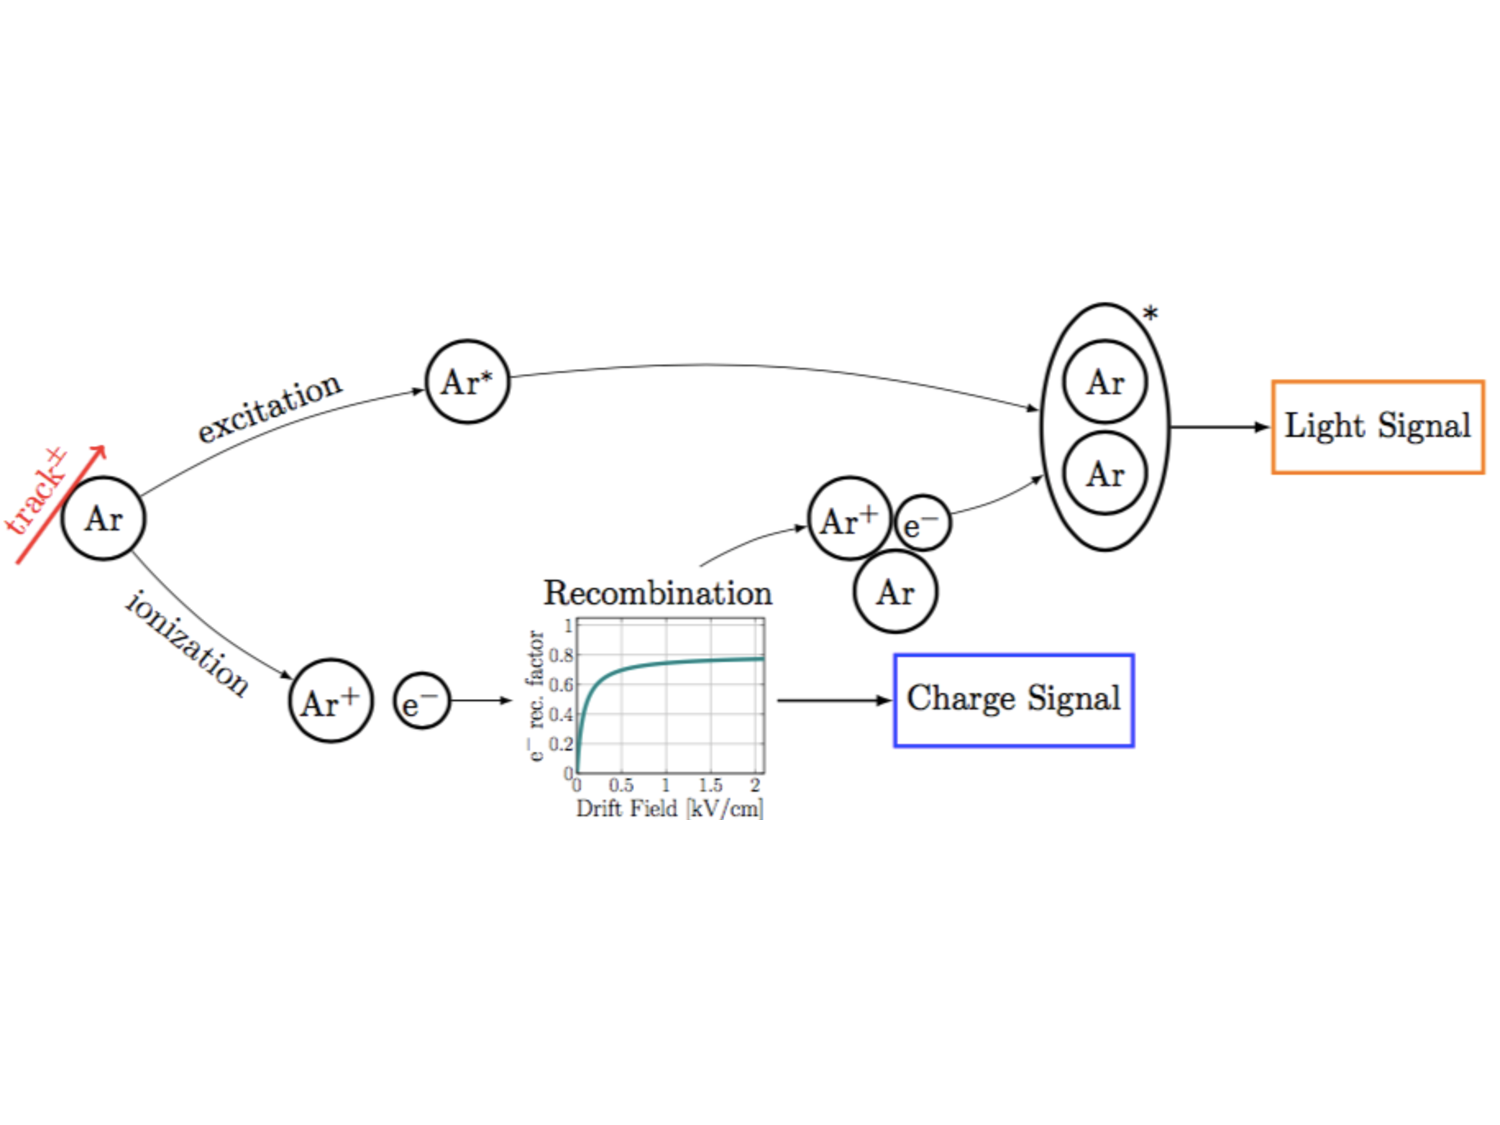
\includegraphics[width=0.9\columnwidth]{pds-scintAr-dppd_6_0.pdf}
\end{dunefigure}
%\{end the part of "principle of operation" that moves to intro. This next part is design considerations. (anne)}

\subsection{Design Considerations}
\label{sec:fdsp-pd-des-consid}

%\todo{\color{blue} Content: Segreto/Warner/Mualem}
%rjw 11/23/18 Add an intro
This section outlines the physical design considerations for a \dword{pds} 
to operate in a \lartpc and introduces the four major components of the \dword{pds} listed in Table~\ref{tab:pds-config-scope}. %, the light collectors, the silicon photosensors, the electronics, and the calibration and monitoring system.

%from sec n.2
The principal task of the \dword{spmod} \dword{pds} is to measure the \dword{vuv} scintillation light produced by ionizing tracks in the TPC within the geometrical constraints of the \dword{apa} structure. The modular arrangement of the \dword{spmod} calls for a configuration across the width of the cryostat starting with an \dword{apa} plane against one cryostat wall, and following with \dword{apa}s and \dword{cpa}s in the order  APA-CPA-APA-CPA-APA. %This means that t
%The central \dword{apa} collect charge and see scintillation light from \lar volumes on both sides, whereas those by the wall collect from only one side. 

The \dwords{pd} must fit within the innermost wire planes of the \dword{apa}s and be  installable through slots in a (wound) \dword{apa} frame (see Chapter~\ref{ch:fdsp-apa}).  Individual \dword{pd} modules are restricted to a profile of dimensions \SI{2.3}{cm} $\times$ \SI{11.8}{cm} $\times$ \SI{209.7}{cm}.  Ten \dword{pd} modules per \dword{apa} for a total of \num{1500} per \dword{spmod}.  Of these, \num{500} are mounted in central \dword{apa} frames and must collect light from both directions (dual-face), and \num{1000} are mounted in frames  near the vessel walls and collect light from only one direction (single-face).

Figures~\ref{fig:apa-frame-pds} and~\ref{fig:pds-pd-full-module} illustrate the baseline configuration of \dwords{pd} and \dword{apa}s in a \dword{spmod}. 


\begin{dunefigure}[Arrangement of APAs in an \dword{spmod} and position of PD modules in APA frame]{fig:apa-frame-pds}
{Left: End-on schematic view of the active argon volume showing the four drift regions and anode-cathode plane ordering of the TPC inside the \dword{spmod}. The three rows of \dword{apa}s are two high and 25 deep. Right: Schematic of an \dword{apa} frame (on its side) showing the ten \dword{pd} modules (vertical in figure). Notice the five slots on the frame's side (top of figure) that they fit through. The other five slots are on the frame's other side, at the bottom of the figure.}
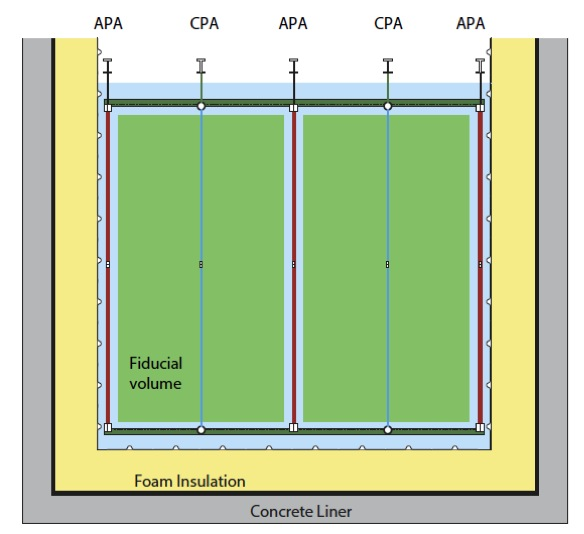
\includegraphics[width=0.45\textwidth]{sp-apa-dune-sp-end-view.jpg}\hspace{0.01\textwidth}
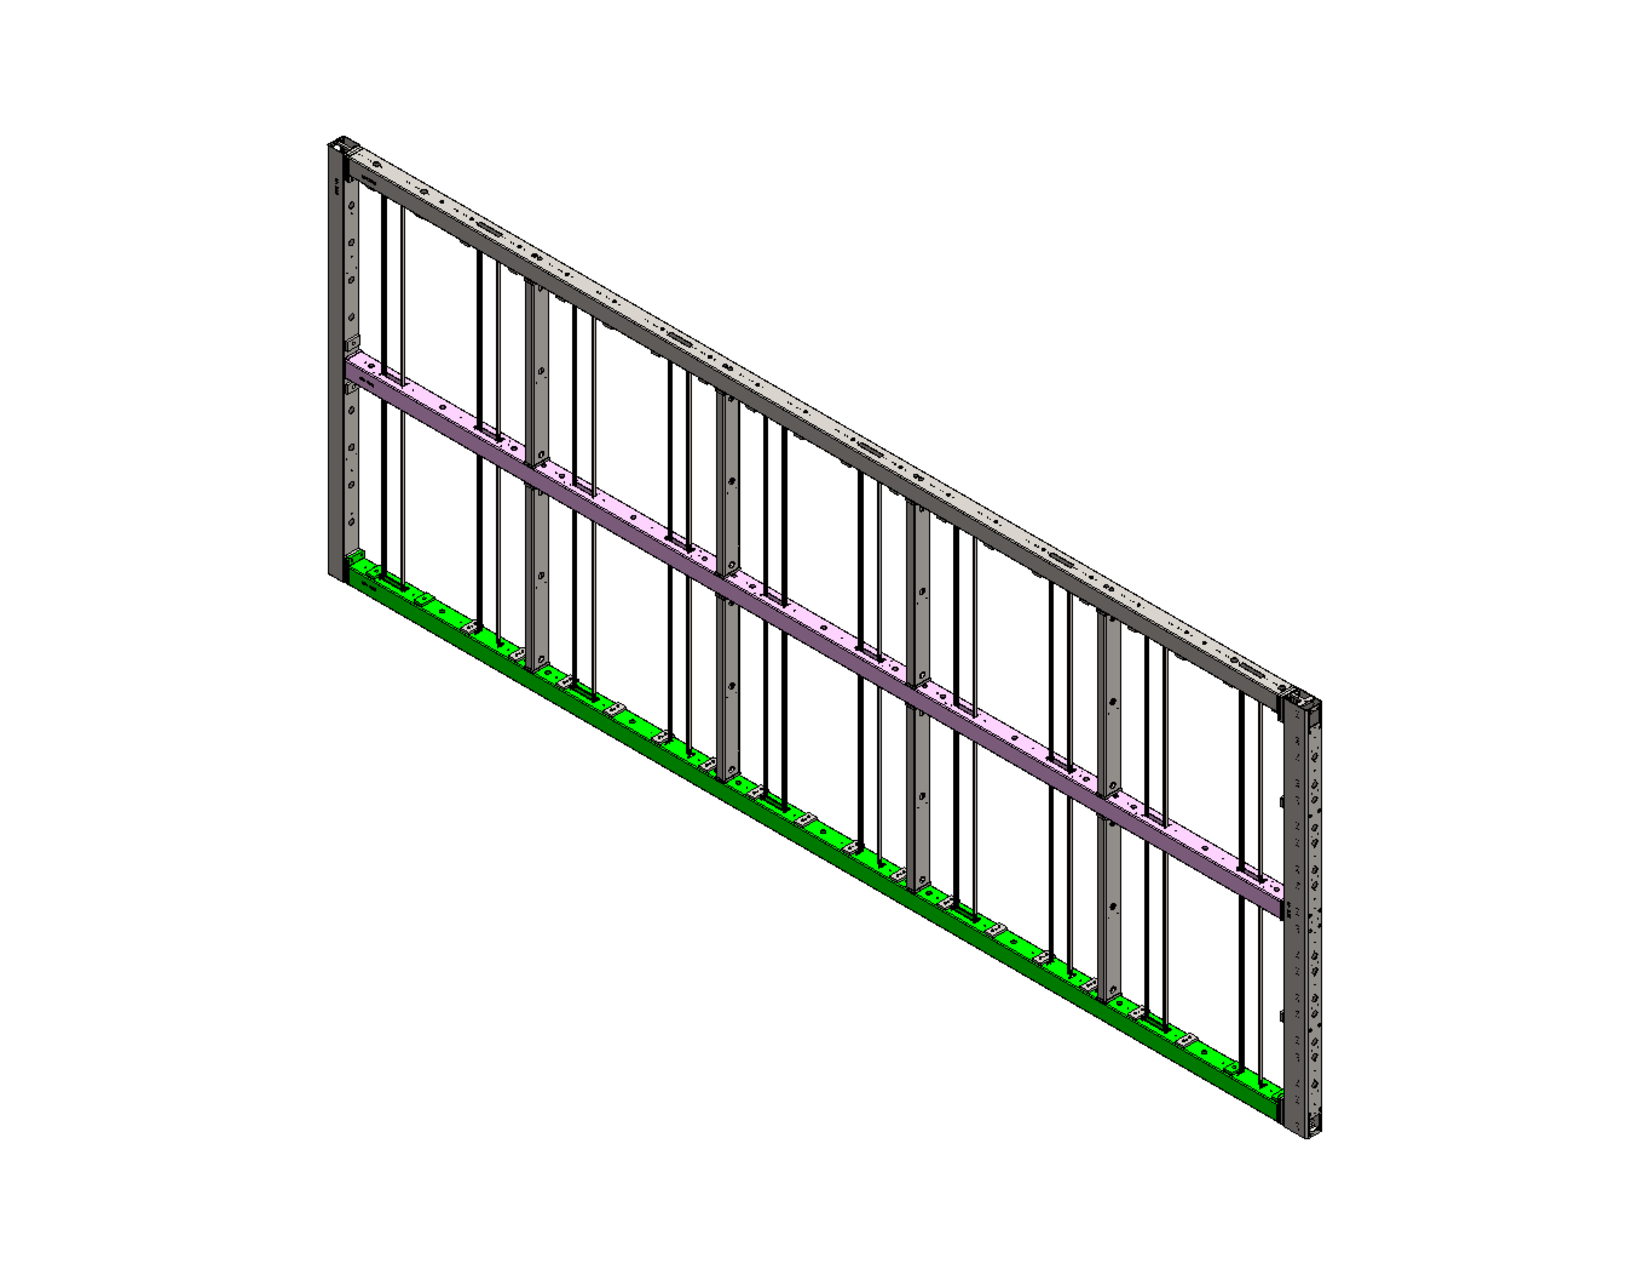
\includegraphics[width=0.45\textwidth]{sp-apa-frame-full-2.pdf}
\end{dunefigure}


\begin{dunefigure}[Geometry of a \dword{pd} module]
{fig:pds-pd-full-module}
{Left: Geometry of a \dword{pd} module. It fits through the \dword{apa} slots, spanning the \dword{apa} width, and holds 24 individual light collector boxes (cells).  Right: A single cell.}
% 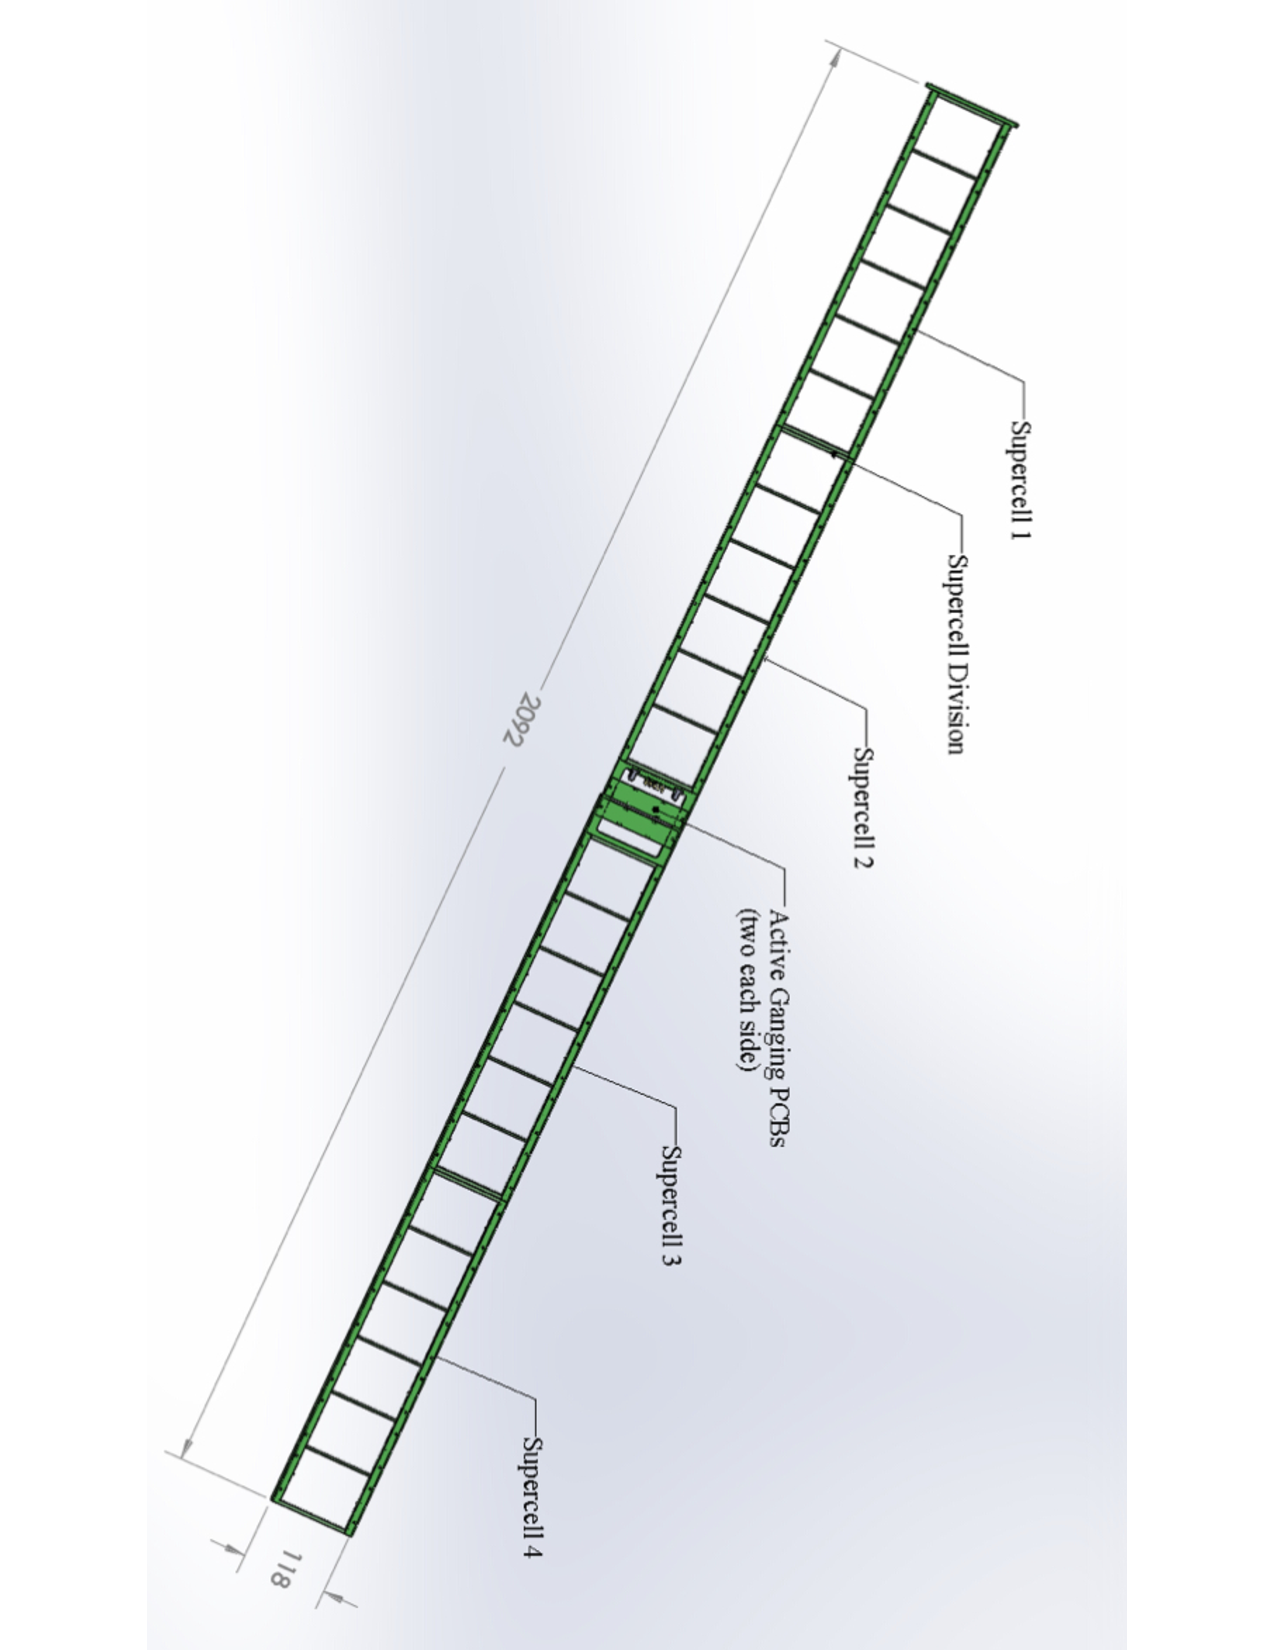
\includegraphics[angle=90,height=.355\textwidth]{pds-design-full-module-dimensioned}
% 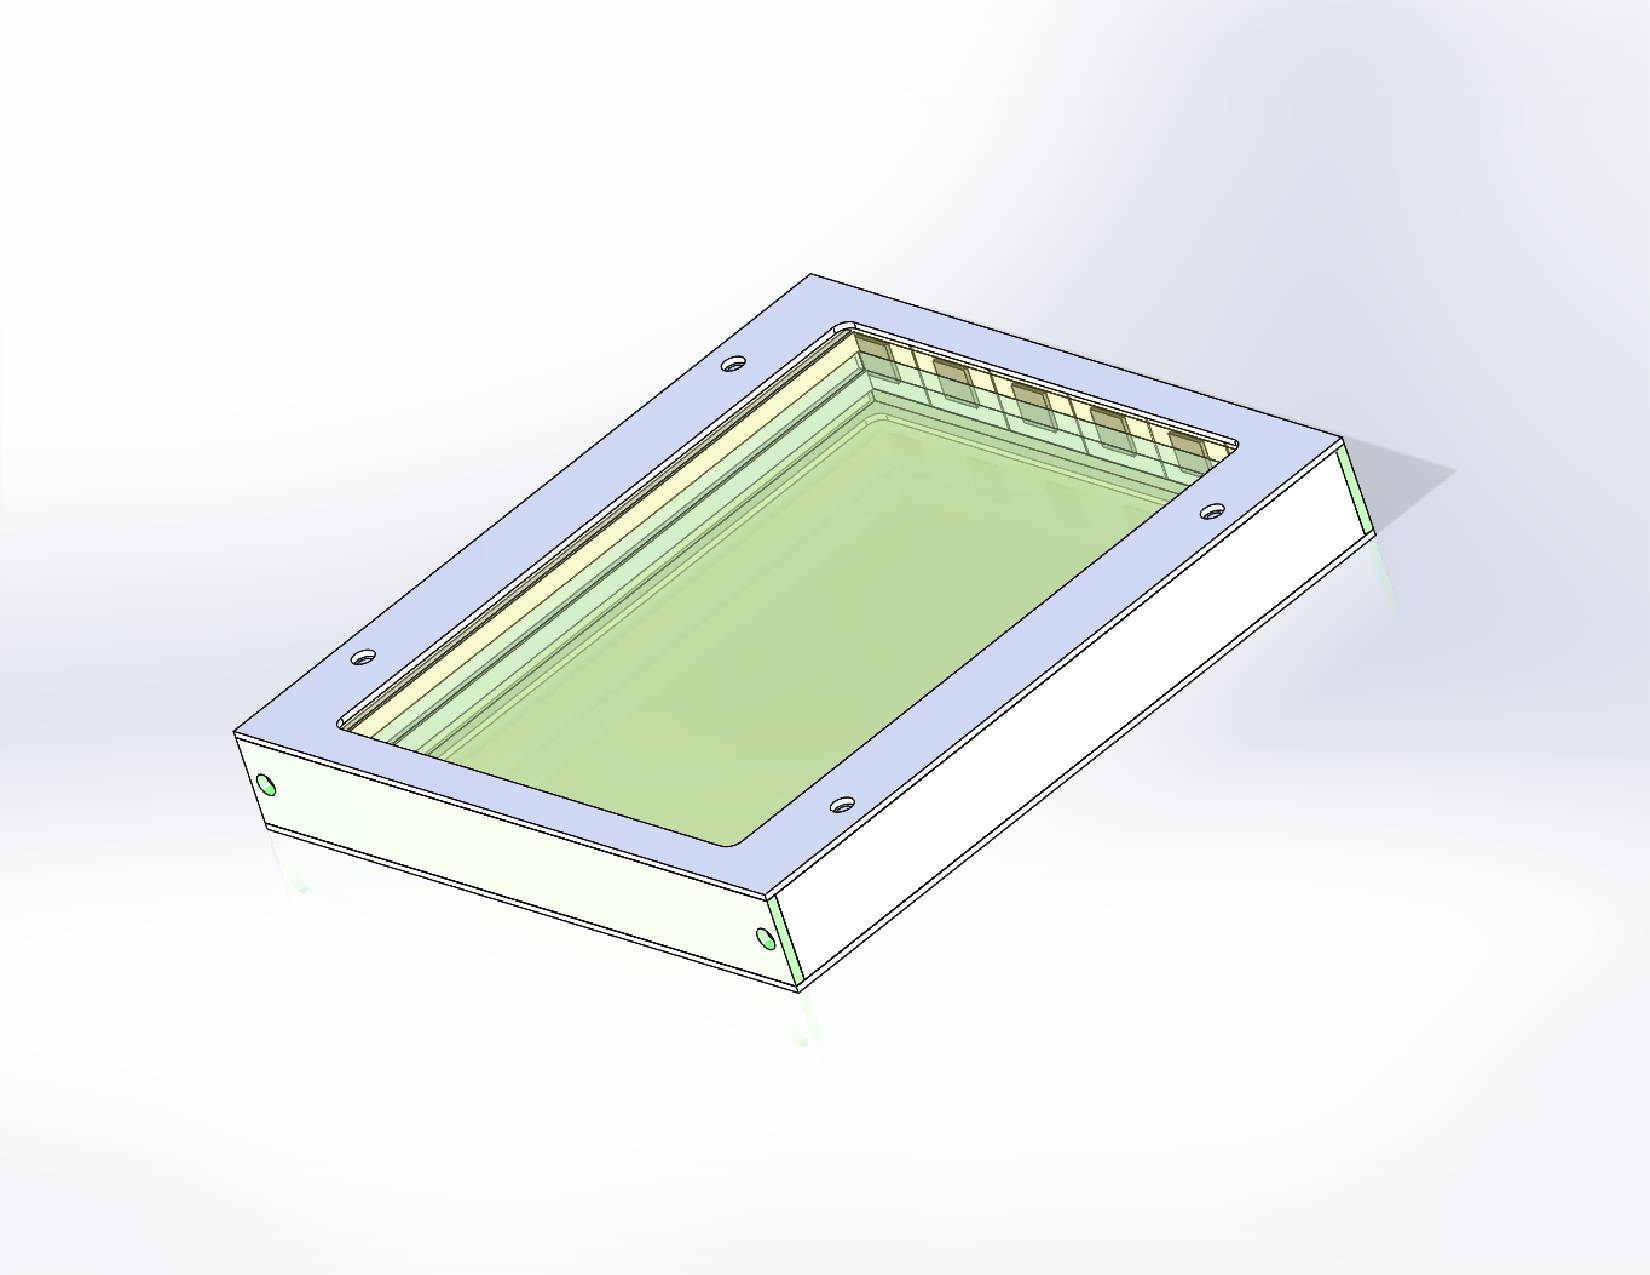
\includegraphics[height=.3\textwidth]{pds-x-arapuca-cell}
 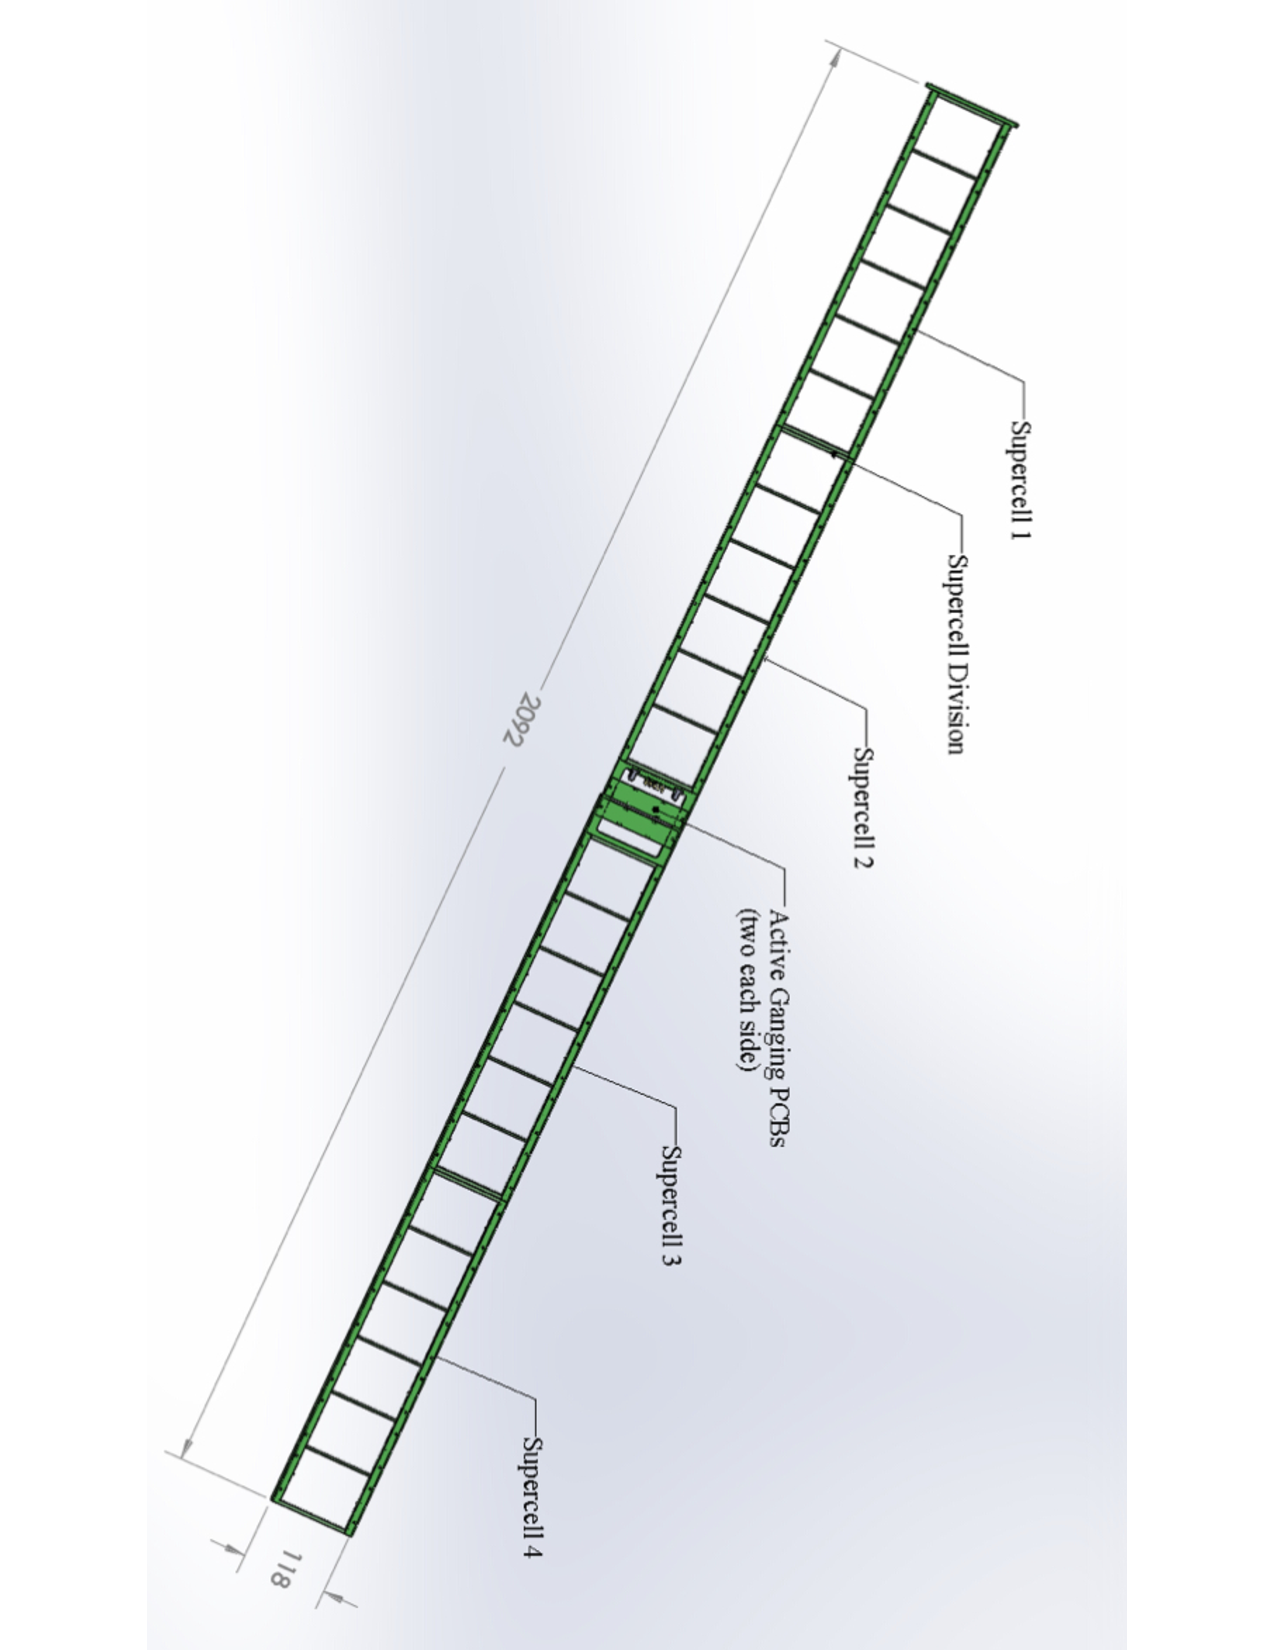
\includegraphics[angle=90,width=0.7\textwidth]{pds-design-full-module-dimensioned}
 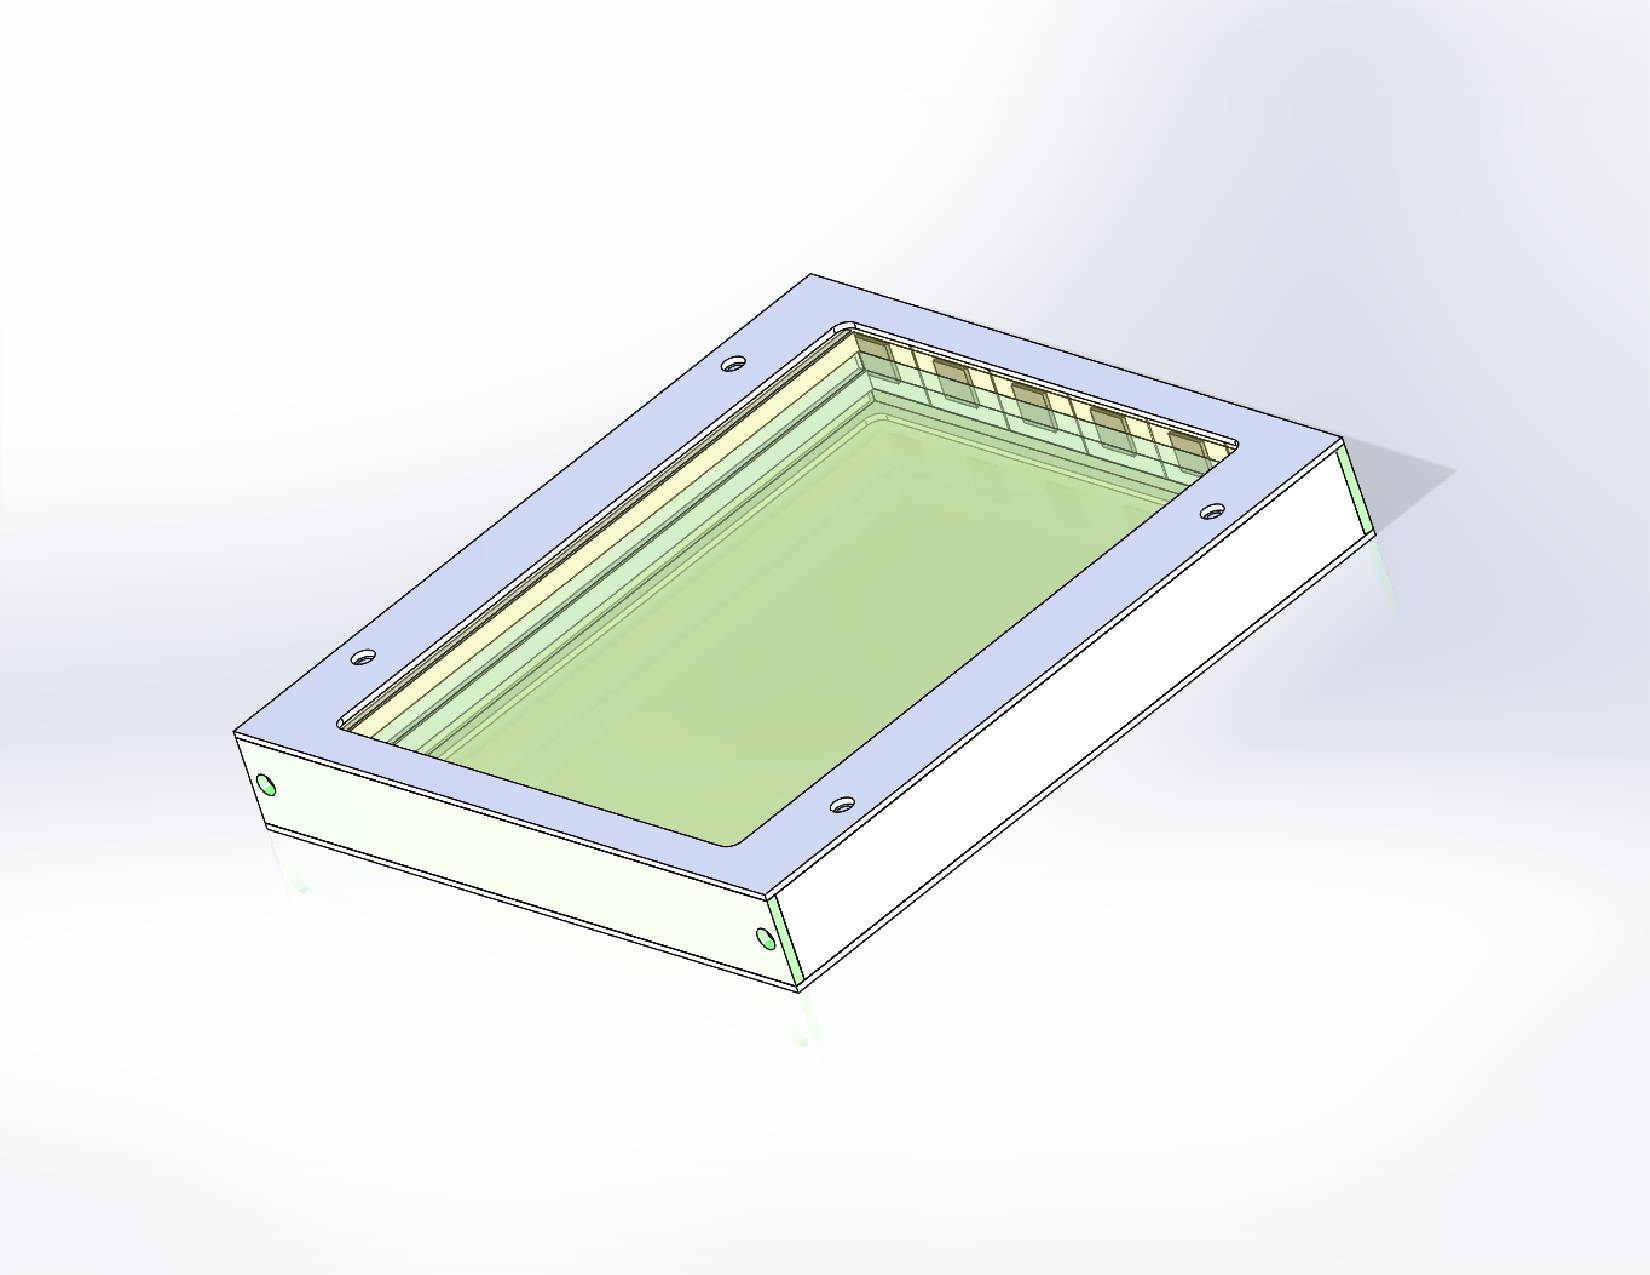
\includegraphics[width=0.25\textwidth]{pds-x-arapuca-cell}
\end{dunefigure}

It is most cost-effective for the \dword{pds} in a massive \lartpc like the \dword{spmod} to collect scintillation light from large areas and channel it 
efficiently towards much smaller photosensors that produce an electrical signal. 
This paradigm %for the detection of \lar scintillation light 
depends on the use of chemical wavelength shifters since most commercial cryogenic large area photosensors currently available are not directly sensitive to \dword{vuv} radiation. This is primarily due to the lack of transparency of fused silica and glass optical windows. 

The most widely used wavelength shifter for \lar detectors is \dword{tpb}\footnote{1,1,4,4-Tetraphenyl-1,3-butadiene, supplier: Sigma-Aldrich\textregistered{}, \url{https://www.sigmaaldrich.com/}.}, which absorbs \dword{vuv} photons and re-emits them with a spectrum centered around \SI{420}{nm}, close to %where most commercial photosensors have their maximum quantum efficiency for photoconversion.
the wavelength of maximum quantum efficiency for photoconversion in most commercial photosensors. 
%rjw 11/223/18 Remove the following - what matters at this stage are the measurements we are doing with our prototypes and how those are modeled in our simulations 
%Though \dword{tpb} has been utilized quite extensively with great success, there are recent publications that warrant caution. For example, until recently the conversion efficiency of \dword{tpb} in coating was taken to be high, approaching or even exceeding \num{100}\% (possible by multi-photon emission), however a recent arXiv paper~\cite{Benson:2017vbw} refutes this previous frequently referenced result. Using much of the same equipment but replacing a damaged reference photodiode, the authors (including an author of the previous paper) report a measurement for the quantum efficiency of \num{40}\% for incident \SI{127}{nm} light. 

%%rjw 11/23/18 we may want to use this reference later in the x-arapuca section 
%Another recent paper\cite{Asaadi:2018ixs} reports that some methods used to coat surfaces with \dword{tpb} suffered loss of the \dword{tpb} coating in \lar, whereas there is no measurable effect if the fluor is dissolved in a polymer matrix. These developments will be followed carefully and highlight the importance of the ongoing R\&D and prototype program.

%\dword{tpb} conversion efficiency is known to be high, there is evidence that it approaches 100\% but reliable direct confirmation of this is not available in the literature\cite{Benson:2017vbw}. - april 2018
%Benson, V. Gehman et al. Retraction of earlier VG work - off by a factor of three due to bad reference photodiode! 
% Old paper VG with wrong results: Fluorescence Efficiency and Visible Re-emission Spectrum of Tetraphenyl Butadiene Films at Extreme Ultraviolet Wavelengths - Nucl.Instrum.Meth. A654 (2011) 116-121
%Tetraphenyl Butadiene Emanation and Bulk Fluorescence from Wavelength Shifting Coatings in Liquid Argon - 	arXiv:1804.00011 [physics.ins-det] April 2018


%The physical dimension of the \dword{pd} system is constrained by the need to fit within the innermost wire planes of the \dwords{apa} and to be installed through slots in the \dword{apa} mechanical frame after it is wound (see Chapter~\ref{ch:fdsp-apa}).  Individual \dword{pd} modules will be restricted to be within an envelope in the form of a long, thin box with dimensions \SI{2.3}{cm} $\times$ \SI{11.8}{cm} $\times$ \SI{209.7}{cm}.  There will be ten \dword{pd} modules per \dword{apa}, for a total of \num{1500} modules.  Of these, \num{500} will be mounted in central APA frames and will require the ability to collect light from both directions, and \num{1000} will be mounted in APA frames mounted near the vessel walls and will only require light collection from one direction.

%\fixme{anne moved the following from the sipm overview section 12/29. Nothing was here for sipms.}
Because of the size constraints imposed by the \dword{apa}, in each light collector concept considered for the \dword{spmod}  
a compact silicon photosensor rather than a traditional photomultiplier must be used to perform the final stage of converting a visible wavelength photon into an electrical signal. 
Distinct from most previous HEP applications of these devices, they must operate reliably for many years at \lar temperatures. 
Experience with a promising early candidate that failed in later batches due to an unadvertised change in the fabrication process emphasizes the importance of a multi-source approach with active engagement of potential vendors to develop a device expressly for cryogenic operation.  


%\{Need a reference for the Ar39 abundance - 
%P. Benetti et al., WARP Collaboration, Nucl. Instr. and Meth. A 574 (2007) 83. 
%Anne asks: natural abundance of X with activity of Y? ``Natural abundance'' seems to need some quantifying... } -- done rjw
A final but significant consideration for the \dword{pds} design is the presence in the \lartpc of the long-lived cosmogenic radioisotope \Ar39, which has a specific activity in argon extracted from the atmosphere of approximately \SI{1}{Bq/kg}~\cite{bkds}. The isotope undergoes beta decay %with 
at a mean beta energy of \SI{220}{keV} with an endpoint of \SI{565}{keV}, and makes up $\sim$70\% of the radiological background signal.
In the \SI{10}{kt} \dword{fd} modules this leads to a rate of more than \SI{10}{MHz} of very short ($\sim$\SI{1}{mm}) tracks uniformly distributed throughout the module, each of which produces several thousand \dword{vuv} scintillation photons. This continuous background impacts the \dword{daq}, trigger, and spatial granularity required of the \dword{pds}.
% rjw Wiki has ($1.01\pm0.08$) Bq/kg, but 1 is good enough for the purpose here.

%%%%%%%%%%%%%%%%%%%%%%%%%%%%%%%%%
\subsection{Design Specifications}
\label{sec:pds:des-specs}
% Source document for the tables is docDB 6422 DUNE Far Detector Single Phase Photon Detector

\fixme{new spec table; content that follows needs revising.}
% This file is generated, any edits may be lost.

\begin{longtable}{p{0.14\textwidth}p{0.13\textwidth}p{0.18\textwidth}p{0.22\textwidth}p{0.20\textwidth}}
\caption{Specifications for SP-PDS \fixmehl{ref \texttt{tab:spec:SP-PDS}}} \\
  \rowcolor{dunesky}
       Label & Description  & Specification \newline (Goal) & Rationale & Validation \\  \colhline

   \newtag{SP-FD-1}{ spec:min-drift-field }  & Minimum drift field  &  $>$\,\SI{250}{ V/cm} \newline ( $>\,\SI{500}{ V/cm}$ ) &  Lessens impacts of $e^-$-Ar recombination, $e^-$ lifetime, $e^-$ diffusion and space charge. &  ProtoDUNE \\ \colhline
    
   
  \newtag{SP-FD-2}{ spec:system-noise }  & System noise  &  $<\,\SI{1000}\,e^-$ &  Provides $>$5:1 S/N on induction planes for  pattern recognition and two-track separation. &  ProtoDUNE and simulation \\ \colhline
    
   
  \newtag{SP-FD-3}{ spec:light-yield }  & Light yield  &  $>\,\SI{20}{PE/MeV}$ (avg), $>\,\SI{0.5}{PE/MeV}$ (min) &  Gives PDS energy resolution comparable that of the TPC for 5-7 MeV SN $\nu$s, and allows tagging of $>\,\SI{99}{\%}$ of nucleon decay backgrounds with light at all points in detector. &  Supernova and nucleon decay events in the FD with full simulation and reconstruction. \\ \colhline
    
    \\ \rowcolor{dunesky} \newtag{SP-FD-4}{ spec:time-resolution-pds } & Name: Time resolution \\
    Description & The time resolution of the photon detection system shall be less than 1 microsecond in order to assign a unique event time.   \\  \colhline
    Specification (Goal) &  $<\,\SI{1}{\micro\second}$  ( $<\,\SI{100}{\nano\second}$ ) \\   \colhline
    Rationale &   Enables \SI{1}{mm} position resolution for \SI{10}{MeV} SNB candidate events for instantaneous rate $<\,\SI{1}{m^{-3}ms^{-1}}$.  \\ \colhline
    Validation &   \\
   \colhline

   \newtag{SP-FD-5}{ spec:lar-purity }  & Liquid argon purity  &  $<$\,\SI{100}{ppt} \newline ($<\,\SI{30}{ppt}$) &  Provides $>$5:1 S/N on induction planes for  pattern recognition and two-track separation. &  Purity monitors and cosmic ray tracks \\ \colhline
    
    \\ \rowcolor{dunesky} \newtag{SP-FD-15}{ spec:lar-n-contamination } & Name: LAr nitrogen contamination \\
    Description & The nitrogen contamination in the LAr shall remain below 25 ppm in order not to significantly affect the number of photons that reach the detectors (for both fast and late light components).   \\  \colhline
    Specification &  $<\,\SI{25}{ppm}$ \\   \colhline
    Rationale &   Maintain \SI{0.5}{PE/MeV} PDS sensitivity required for triggering proton decay near cathode.  \\ \colhline
    Validation & In situ measurment  \\
   \colhline


    \\ \rowcolor{dunesky} \newtag{SP-PDS-1}{ spec:ly-uniformity } & Name: Light yield uniformity within the active volume. \\
    Description & The light yield in even the dimmest regions of the detector shall be sufficient to correctly associate scintillation light with events with energy > 200 MeV with efficiency >\SI{99}{\%}. The goal is to dramatically improve the uniformity to improve background rejection, triggering efficiency, and energy resolution.   \\  \colhline
    Specification (Goal) &  $>\,\SI{0.5}{pe/MeV}$  ( >\SI{4}{pe/MeV} ) \\   \colhline
    Rationale &   Fiducializing nucleon decay backgrounds with  $>\,\SI{99}{\%}$ efficiency at all points in the detector.  \\ \colhline
    Validation & Simulated nucleon decay events in the far detector.  \\
   \colhline

    \\ \rowcolor{dunesky} \newtag{SP-PDS-2}{ spec:spatial-localization } & Name: Spatial localization \\
    Description & Events inside the active volume shall be localized in the Y-Z plane  to within < \SI{2.5}{\meter} using light signals.   \\  \colhline
    Specification &  < \SI{2.5}{\meter} \\   \colhline
    Rationale &   Enables more accurate matching of photon detector and TPC signals.  \\ \colhline
    Validation & Supernova neutrino and nucleon decay simulation in the far detector.  \\
   \colhline

    
   
  \newtag{SP-PDS-3}{ spec:env-light-exposure }  & Environmental light exposure  &  \num{0} sunlight.  All other unfiltered sources: $<\,\num{30}$ minutes integrated across all exposures &  Prevent damage to wavelength-shifting coatings due to UV exposure &  ProtoDUNE, IU studies \\ \colhline
    
    \\ \rowcolor{dunesky} \newtag{SP-PDS-4}{ spec:env-humidity-limit } & Name: Environmental humidity limit \\
    Description & All working environments with exposed TPB coatings must maintain <\SI{50}{\%} Relative Humidity (RH) at  \SI{70}{\degree F}.   \\  \colhline
    Specification (Goal) &  < \SI{50}{\%} RH at \SI{70}{\degree F}  ( ALARA ) \\   \colhline
    Rationale &     \\ \colhline
    Validation &   \\
   \colhline

   
  \newtag{SP-PDS-5}{ spec:light-tightness }  & Light-tight cryostat  &  Cryostat light leaks responsible for $<\,\SI{10}{\%}$  of data transferred from PDS to DAQ &  Minimizing false triggers due to cryostat light leaks helps limit the data transfer rate to  \dshort{daq}. &  \dshort{pdsp} and \dshort{iceberg} \\ \colhline
    
   
  \newtag{SP-PDS-6}{ spec:ed-light }  & Light from electrical discharge  &  Light generated by HV system responsible for $<\,\SI{10}{\%}$ total trigger rate in DAQ &  Minimizing false triggers due to corona light from \dword{hv} discharge helps limit the data transfer rate to the \dword{daq}. &  \dword{pdsp} and \dword{iceberg} \\ \colhline
    
    \\ \rowcolor{dunesky} \newtag{SP-PDS-7}{ spec:mech-deflection } & Name: Mechanical deflection (static) \\
    Description & The PDS shall not deviate more than 5mm from nominal position in any APA orientation due to PD load   \\  \colhline
    Specification &  $<\,\SI{5}{\milli\meter}$ \\   \colhline
    Rationale &   Constrain PD motion (static and dynamic load) to avoid damaging APA  \\ \colhline
    Validation & PD FEA, ProtoDUNE, ICEBERG, Ash River integration tests, CERN pre-production integration test  \\
   \colhline

    \\ \rowcolor{dunesky} \newtag{SP-PDS-8}{ spec:apa-install } & Name: Clearance for installation through APA side tubes \\
    Description & PD modules must fit and be secured to the APA through slots in one side of the APA, as designed in concert with APA group.   \\  \colhline
    Specification &  $>$\SI{1}{\milli\meter} \\   \colhline
    Rationale &     \\ \colhline
    Validation &   \\
   \colhline

   
  \newtag{SP-PDS-9}{ spec:mech-compatibility }  & No mechanical interference with APA, SP-CE and SP-HV detector elements (clearance)  &  $>\,\SI{1}{\milli\meter}$ &  PD mounting and securing element tolerances must prevent interference with APA and CE cable bundles. &  Validation will occur in \dword{iceberg}, Ash River integration  tests, and the \dword{cern} pre-production integration tests. \\ \colhline
    
   
  \newtag{SP-PDS-10}{ spec:pds-cable }  & APA intrusion limit for PD cable routing   &  $<\,\SI{6}{\milli\meter}$ &  \dword{pd} modules must install into \dword{apa} frames following wire wrapping.  \dword{pd} modules must not occlude \dword{apa} side tubes. &  \dword{iceberg}, Ash River integration  tests, and the CERN pre-production integration tests \\ \colhline
    
   
  \newtag{SP-PDS-11}{ spec:pds-cablemate }  & PD cabling cannot limit upper-lower APA junction gap  &  \SI{0}{\milli\meter} separation mechanically allowed &  PD cable connections must not limit the minimum upper and lower APA separation. &  Validation will occur in \dword{iceberg}, Ash River integration  tests, and the \dword{cern} pre-production integration tests. \\ \colhline
    
   
  \newtag{SP-PDS-12}{ spec:pds-clearance }  & Maintain PD-APA clearance at LAr temperature.   &  $>\,\SI{0.5}{\milli\meter}$ &  \dword{pd} mounting frame and cable harness must accommodate thermal contraction of itself and \dword{apa} frame. &  Thermal modeling, \dword{protodune}, \dword{iceberg}, \dword{cern} pre-production integration tests \\ \colhline
    
   
  \newtag{SP-PDS-13}{ spec:pds-datarate }  & Data transfer rate from SP-PD to DAQ  &  $<\,\SI{8}{Gbps}$ &  \dword{pd} data transfer must not exceed \dword{daq} data throughput capability. &  Maximum bandwidth out of the \dword{pd} electronics is \SI{80}{Mbps} \\ \colhline
    
    \\ \rowcolor{dunesky} \newtag{SP-PDS-14}{ spec:pds-signaltonoise } & Name: Signal-to-noise in SP-PD \\
    Description & The signal-to-noise ratio (single PE pulse height / baseline noise RMS) shall be greater than 4.   \\  \colhline
    Specification &  $>4$ \\   \colhline
    Rationale &     \\ \colhline
    Validation &   \\
   \colhline

   
  \newtag{SP-PDS-15}{ spec:pds-darkrate }  & Dark noise rate in SP-PD  &  $<\,\SI{1}{kHz}$ &  Keep data rate within electronics bandwidth limits. &  Pre-production photosensor testing, \dword{pdsp}, \dword{iceberg} and \dword{pdsp2} \\ \colhline
    
   
  \newtag{SP-PDS-16}{ spec:pds-dynamicrange }  & Dynamic Range in SP-PD  &  $<\,\SI{20}{\%}$ &  Keep the rate of saturating channels low enough for effective mitigation. &  Pre-production photosensor testing, \dword{pdsp}, \dword{iceberg} and \dword{pdsp2} \\ \colhline
    


\label{tab:specs:SP-PDS}
\end{longtable}

We distinguish two levels of %requirements 
specifications for the \dword{pds} necessary to achieve the DUNE science objectives. The first %consists of the requirements on the 
relates to measurement of physical parameters associated with events of scientific interest such as the event time and the energy of the observed particles. The second concerns %the specifications for 
the detector hardware performance required to make those measurements, such as the sensitivity to the produced light signal per unit of deposited energy (light yield). 

Table~\ref{tab:pds-sys-req} summarizes the first level %requirements
specifications: 
\fixme{This text will change when the final table goes in (Anne)}
The first row attempts to ensure high efficiency and good energy resolution for proton decay and atmospheric neutrinos.  The second row establishes that a timing measurement is required for event localization (in conjunction with the TPC drift time measurement) and targets core collapse \dword{snb} neutrinos. The third row identifies that there much be sufficient dynamic range in the electronics to over the range of energy deposition of all events of science interest. The final row describes a measurement \textit{goal} that the collaboration believes would extend the capability of the system but is not considered a requirement to achieve the core science goals. Specifically, we establish a goal to measure the energy in scintillation light from \dword{snb} events near the peak of the spectrum ($\sim$\SI{20}{MeV}) with a precision similar to that of the ionization measurement. 
The combined measurement of ionization charge and scintillation light has been shown to improve the determination of the energy deposition of an event. 
% Per study by Bishu 12/3/18  rjw
We note that the smearing of the observed charged particle energy due the physics of the neutrino interaction (such as unobserved neutrons) is $\sim$18\% at the peak of the spectrum.
%In the past year, the potential for \lar scintillation light to contribute to the energy reconstruction of events has recently been recognized, in particular for lower energy events such as from \dwords{snb}(\num{10}-\SI{100}{MeV}). 
%In response, the collaboration has established 

%Table~\ref{tab:pds-det-req} IDR table
Tables~\ref{tab:spec:time-resolution} and \ref{tab:spec:light-yield} show the primary \dword{pds} performance specifications that correspond to the event measurement requirements.
%the corresponding photon detection light yield, timing and spatial separation requirements. 
%To achieve a \num{15}\%  calorimetric measurement with light requires approximately ten times higher light yield for the \dword{pds} than the baseline requirement. 
%\{updated language and rationale for baseline option} %rjw 11/223/18

In Section~\ref{sec:fdsp-pd-design} we present a design that meets or exceeds the specifications while respecting the significant constraints imposed by the physical structure and size of the \dword{spmod}. Section~\ref{sec:fdsp-pd-validation} summarizes an extensive set of prototypes that provide validation of the assumptions used in the design and the results of simulations that establish relationships between the performance specifications and the measurement requirements of Table~\ref{tab:pds-sys-req}. 

%%%%%%%%%%%%%%%%%%%%%%%%%%%%%%%%%%%%%%%%%%%%%%%%%%%%%%%%%%%%%%%%%%%%%%%%%%%%
%% rjw 1/12/19 Waiting for final word on  what specifications tables are allowed i.e. use only the autogenerated tables and remove the measurement specifications and goals with more text ones below 
%%%%%%%%%%%%%%%%%%%%%%%%%%%%%%%%%%%%%%%%%%%%%%%%%%%%%%%%%%%%%%%%%%%%%%%%%%%%

%\begin{dunetable}
%[Key performance requirements for the PD system (Note: these are under review).]
%{cc}
%{tab:pds-req}
%{Highest-level PD performance requirements to achieve the detection efficiency of $90$\% for energy deposit of \SI{> 200}{MeV}\{what is the origin of this requirement - docDB indicates 1 pe/MeV at the center of the TPC} } 
%Requirement  & Value \\ \toprowrule
%Light Yield  & \SI{0.1}{pe/MeV} for events near the cathode plane  \\ \colhline
%Timing Resolution & \SI{1}{$\mu$s}   \\ \colhline
%\end{dunetable}
% rjw Requirements extracted from the global science and FD engineering requirements documents docDB 112}

%\fixme{(For now at least) Keep the summary table of PDS science objective table used in IDS since it is PD detector independent and put the PD performance specification in the separate autogenerated entries in the docDB 6422 requirements spreadsheet.  rjw 20/11/18}

%\fixme{In table\ref{tab:pds-sys-req} I changed the PD energy measurement resolution goal 10\%->15\% -- make this consistent with official Specification spreadsheet and any justification statements elsewhere. After some exchanges with Alex - this is justified also in terms of the inherent spread in visible energy in neutrino interactions at energies near the SNB nu spectrum peak - added some text in the simulation section.}

\begin{dunetable}
[\Dword{pds} measurement specifications and goals.]
{p{0.45\textwidth}p{0.45\textwidth}}
{tab:pds-sys-req}
{\dword{pds} measurement specifications and goals. \fixme{replace (Anne)}}
Specification  	& Rationale \\ \toprowrule
The  \dword{fd} \dword{pds} shall detect sufficient light from events depositing visible energy >\SI{200}{MeV} to efficiently measure the time and total intensity. 
			& This is the region for nucleon decay and atmospheric neutrinos. The time measurement is needed for event localization for optimal energy resolution and background rejection.			\\ \colhline
The  \dword{fd} \dword{pds} shall detect sufficient light from events depositing visible energy <\SI{200}{MeV} to provide a time measurement.  The efficiency of this measurement shall be adequate for \dword{snb} events. 
			& Enables low energy measurement of event localization for \dword{snb} events. The efficiency may vary significantly for visible energy in the range \SI{5}{MeV} to \SI{100}{MeV}. 		\\ \colhline
The \dword{fd} \dword{pds} readout electronics shall record time and signal amplitude from the photosensors with sufficient precision and range to achieve the key physics parameters. 
			& The resolution and dynamic range needs to be adjusted so that a few-\phel signal can be detected with low noise.  The dynamic range needs to be sufficiently high to measure light from a muon traversing a TPC module.  \\ \colhline
Goal: The  \dword{fd} \dword{pds} shall detect sufficient light from events depositing visible energy of  \SI{10}{MeV} to provide an energy measurement with a resolution of 15\%. 
			& Enables energy measurement for \dword{snb} events with a precision similar to that from the TPC ionization measurement. \\
\end{dunetable}


%%%%%%%%%%%%%%%%%%%%%%%%%%%%%%%%%%%%%%%%%%%%%%%%%%%%%%%%%%
\subsection{Design Overview} %new sec from anne
\label{sec:pds:des-ov}

%\fixme{from top of old design chapter anne.}
%The light collector design must optimize the costs of various components of the system while meeting the performance requirements.  It will use \dwords{sipm}, which provide a commercially available compact solution for photon measurement.  However, the response of these devices, which typically peaks in the visible range (>\SI{400}{nm}), is not well-matched to incident \SI{127}{nm} scintillation photons, so a wavelength shifter or some sort is required.  In addition, even though production cost and key performance parameters have improved significantly in recent years, covering the light detector surfaces with enough \dwords{sipm} to meet the physics requirements of the \dword{pds} would be cost-prohibitive. The light collector design must optimize the costs of various components of the system while meeting the performance requirements.  

 

%%% rjw 
The  large-area light collectors are the core modular elements of the \dword{pds}.  They 
convert incident \SI{127}{nm} scintillation photons into photons in the visible range (>\SI{400}{nm}) that compact  \dword{sipm} photosensors, in turn,  convert to an electrical signal. The light collector design must optimize the costs of various components of the system while meeting the performance requirements.  %It will use \dwords{sipm}, which provide a commercially available compact solution for photon measurement.  However, the response of these devices, which typically peaks in the visible range (>\SI{400}{nm}), is not well-matched to incident \SI{127}{nm} scintillation photons, so a wavelength shifter or some sort is required.  In addition, e
Even though production cost and key performance parameters of \dwords{sipm} have improved significantly in recent years, covering the light detector surfaces with enough of them to meet the physics requirements of the \dword{pds} would be cost-prohibitive. 
%Since the size and cost of currently available \dwords{sipm} are not well matched to the performance requirements in the large-volume \dword{spmod}, t
The light collector design aims to maximize the active \dword{vuv}-sensitive area of the \dword{pds} while minimizing the necessary photocathode (\dword{sipm}) coverage. This is detailed in
Section~\ref{sec:fdsp-pd-lc}.
%Section~\ref{sec:fdsp-pd-design}. 

% rjw 1/12/19 Note docDB 11644 does not yet have any content!
%Additional details on the design too specialized for the scope of this \dword{tdr} can be found in the DUNE Single-Phase Photon Detector Design Report~\citedocdb{11644}. 
\fixme{The document does not exists yet (it is a placeholder with just a title page); Dave what is the timescale? Should we leave this statement out until it is ready (TB and AH commented out) - or at least give a warning so LBNC doesn't get a surprise if they do look it up?}

%%%%%%%%%%%%%%%%%%%%%
\subsubsection{Light Collectors} 
\label{sssec:photoncollectors}


%In the following we will distinguish between the terms photon \textit{collection} efficiency and photon \textit{detection} efficiency (PDE). Collection efficiency is the number of visible photons delivered to the \dwords{sipm} divided by the number of \dword{vuv} photons incident on the \dword{pd} module active area; this parameter is used to report results of calculations or simulations of predicted device performance independent of the \dword{sipm} used.  Detection efficiency is the number of detected \phel{}s from the \dword{sipm}(s) divided by the number of \dword{vuv} photons incident on the \dword{pd} module active area; this is generally the result of a direct measurement unless the detailed performance of the \dword{sipm} is known and divided out. 
%The effective area of a \dword{pd} module is another useful figure-of-merit that is defined to be the photon detection efficiency multiplied by the photon collecting area of a \dword{pd} module. 

%Numerous \dword{pd} photon collector module options were investigated prior to the formation of the \single \dword{pd} consortium, of which four were selected for further development. 


%\{I moved the "DUNE investigated" text to the validation section and moved the top of the light collector design text  1.2.1 here (anne)}

The \dword{xarapu}, adopted for the baseline design and detailed in 
%Section~\ref{ssec:fdsp-pd-pc-arapuca}, 
Section~\ref{sec:fdsp-pd-lc},
is an evolution of the ARAPUCA concept that combines its light trapping capability with the collection and transport capabilities of light guides.   

The ARAPUCA concept takes advantage of a new approach to \lar scintillation photon detection where the effective detection area is increased by trapping photons inside a flat box (cell) with highly reflective internal surfaces until reflections guide them to active photosensors of relatively small area. 
\dword{xarapu} includes placement of an acrylic wavelength-shifting light guide inside the cell, occupying a portion of the volume. Photons trapped in the light guide are wavelength-shifted and transported to the photosensors via total internal reflection with high efficiency. 

 % \dword{sipm}~\cite{arapuca_jinst}. 

Photon trapping is achieved through a novel use of wavelength-shifting and the technology of the dichroic shortpass optical filter. These commercially available filters are created by using multilayer thin films that %have the property of being 
are highly transparent to photons with a wavelength below a tunable cutoff, %while being 
with transmission typically greater than 95\%, yet almost perfectly reflective to photons with a wavelength above the cutoff.  Such a filter coated with either one or two different wavelength-shifters, depending on the detailed implementation, forms the entrance window to a cell whose internal surfaces are covered by highly reflective acrylic foils
%(3M-Vikuiti ESR \footnote{3M Vikuiti\texttrademark\ ~foils. https://en.wikipedia.org/wiki/Vikuiti.}, for example), 
except for a small fraction occupied by \dwords{sipm}.

%To act as a photon trap, the wavelength-shifter deposited on the outer face of the dichroic filter must have its emission wavelength less than the cut-off wavelength of the filter, below which transmission is typically greater than 95\%. 
For the collector to act as a photon trap, the emission wavelength of the wavelength-shifter deposited on the outer face of the dichroic filter must be less than the cutoff wavelength of the filter. 
%, below which transmission is typically greater than 95\%. 
The transmitted photons pass through the filter where they encounter a second wavelength-shifter %either on the inner surface of the filter or coated on the reflecting inner surfaces of the box, 
with an emission spectrum greater than the cutoff wavelength, thus trapping them. 
%The location of the second wavelength-shifter is different in the single- and dual-face cells.
%In a single-face cell, the filter is coated also on the inside surface with a wavelength shifter; in a dual-face cell
%\fixme{In a single-face cell, the filter is coated also on the inside surface with a wavelength shifter; in a dual-face cell check and come back - Anne}

Trapped photons reflect off the inner walls and the filter surface(s) (of reflectivity typically greater than \SI{98}{\%}) 
and have a high probability of impinging on a \dword{sipm} before being lost to absorption. The concept is illustrated in Figure~\ref{fig:arapuca}\footnote{In the original ARAPUCA concept, the second wavelength-shifter was coated on the inner surface of the filter and the WLS plate shown in the figure was absent.}.
Validation of the ARAPUCA concept is described in Section~\ref{sec:fdsp-pd-validation}.
%It is easy to show that, for small values of \dword{sipm} coverage of the internal surface, the amplification factor is equal to $A=1/(2(1-R))$, where R is the average value of the reflectivity of the internal surfaces; for an average reflectivity of 0.95 the amplification factor is equal to ten.

\begin{dunefigure}[Schematic representation of the \dword{xarapu} operating principle.]{fig:arapuca}
{Schematic representation of the \dword{xarapu} operating principle. This example assumes a filter cutoff of \SI{400}{nm}. [Note: In the original ARAPUCA concept, the second wavelength-shifter was coated on the inner surface of the filter and the WLS plate shown in the figure was absent.]}
%  %\includegraphics[height=5cm]{pds-arpkscheme}   
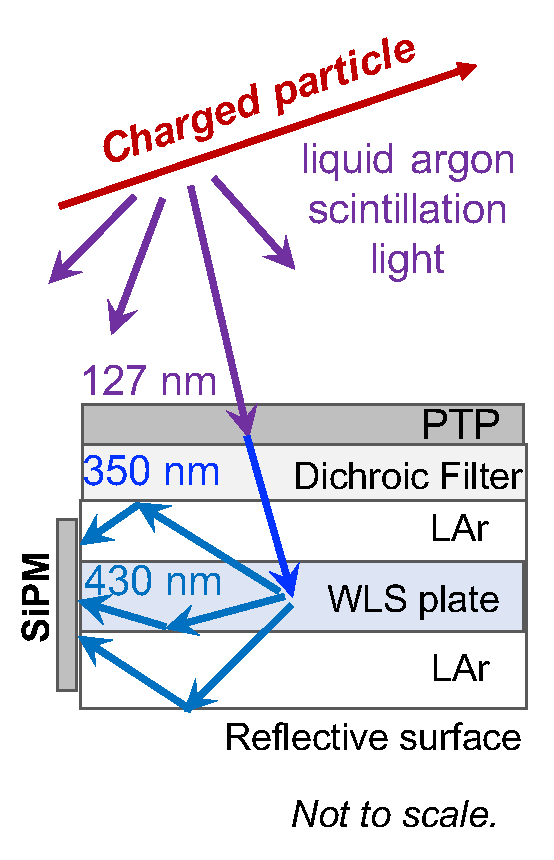
\includegraphics[height=6cm]{pds-x-arapuca-concept}   
\end{dunefigure}

While the ARAPUCA modules deployed in \dword{pdsp} collect light from only one direction, the next generation \dword{xarapu} can be deployed as either single-face or dual-face readout by using either an opaque reflector plate (single) or a second dichroic filter window (dual) on the second face. 
Figure~\ref{fig:3dtpc-pd} shows how a light-collector module is incorporated into an \dword{apa}. An identical modular mounting scheme was used for each of the three options investigated\footnote{Two wavelength-shifter-coated light guide options were also investigated in detail over several years.}. One module spans the width of an \dword{apa}.


\begin{dunefigure}[\threed model of \dwords{pd} in the \dword{apa}.]{fig:3dtpc-pd}
{\threed model of \dwords{pd} in the \dword{apa}. The model on the left shows the full width of the TPC with the configuration APA-CPA-APA-CPA-APA. The figure on the right shows a detail of the top far side of the TPC where three photon collector technologies deployed in \dword{pdsp} are illustrated; the final \dword{detmodule} will contain just \dword{xarapu}.}
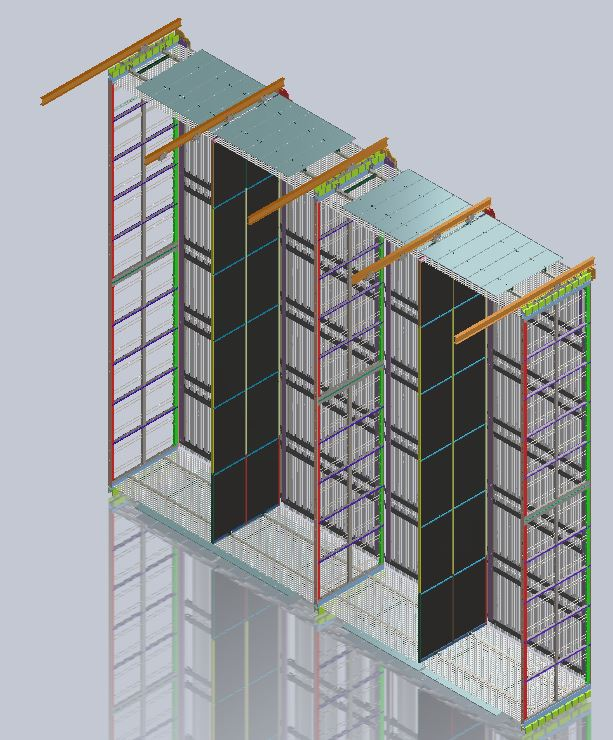
\includegraphics[height=6cm]{pds-dune-sp-tpc-3d.jpg}
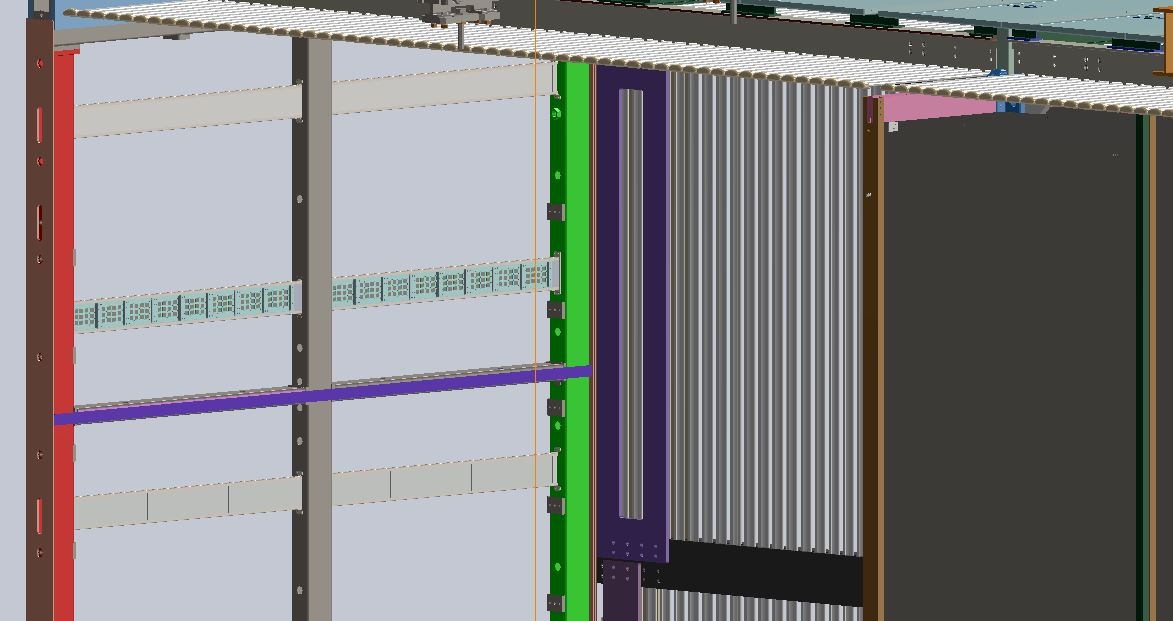
\includegraphics[height=6cm]{pds-dune-sp-tpc-3d-zoom.jpg}
\end{dunefigure}

%\fixme{keep illustration here, move the following to validation or full description in "design" chapter (anne)}

The light collector design has the flexibility to accommodate greater demands, such as might be desired for \dword{sbn} physics, without major changes. One example is to increase the number of \dwords{sipm} to increase light yield, which could be incorporated quite late in the final design stages since it would not involve significant mechanical changes.

%%%%%%%%%%
\subsubsection{Silicon Photosensors} 


The \dword{spmod} \dword{pds} uses a multi-step approach to scintillation light detection with final stage of conversion into electrical charge performed by silicon photomultipliers (\dwords{sipm}). Robust photon detection efficiency, low operating voltages, small size, and ruggedness make their use attractive in the \single design where the photon detectors must fit inside the \dword{apa} frames. 

Based on extensive testing and experience with the vendor, we have selected a \SI{6}{mm}$\times$\SI{6}{mm} \dwords{mppc} % (Multi-Pixel Photon Counters) 
produced by Hamamatsu\footnote{Hamamatsu\texttrademark{} Photonics K.K., \url{http://www.hamamatsu.com/}.} (Japan) as the current baseline \dword{sipm} device. 
We are also vigorously pursuing an alternative based on the design of a device developed for operation in \lar by the DarkSide experiment collaboration and Fondazione Bruno Kessler (FBK)\footnote{Fondazione Bruno Kessler\texttrademark{}, \url{https://www.fbk.eu}.} (Italy).

The baseline \dword{pds} design has 192 \num{6}$\times$\SI{6}{mm$^2$} \dwords{mppc} per \dword{pd} module with groups of 48 \dwords{mppc} electrically ganged into four electronics readout channels. This leads to a total of 288,000 \dwords{mppc} per \dword{spmod}. 



%The size of currently available \dwords{sipm} (typically less than \SI{1}{cm$^2$}) is far smaller than the spatial granularity required for the experiment, so the output of individual devices will be electrically summed (ganged) to reduce the electronics channel count. This could be achieved either by simply connecting together the output of multiple devices, passive ganging, or using active components, active ganging, if the signal is too degraded for the passive approach. An optimal solution could involve a combination of the two approaches. 


%%%%%%%%%%%%%%%%%%%%%%%%%%%%%%%%%%%
\subsubsection{Readout Electronics} 

%\fixme{rjw 11/25/18 Note: This is Design Consideration section so should just be on high level considerations not implementation }
%\fixme{DWW  The mu2e WFD front end electronics are now the baseline.  This sections needs modification--  I think we should mention charge integration, but greatly reduce the prominence.  The last sentence in this paragraph buries the lead.}
%\fixme{modifed below by Djurcic 11/29/18; need further understand what the "summing" baseline and come back here}

%\fixme{12/1/18 rjw added a few words to make it more like Design Considerations, but this should be fleshed out by conveners. (The paragraphs that followed were specifics on using Mu2e rather than SSP so moved to the Design section)}

%The \dword{pds} design requires the electronic readout system to collect and process electric signals from photosensors in \lar  to provide the interface to trigger and timing systems to support data reduction and classification, and to enable data transfer to an offline storage system for physics analysis. The quantitative requirements for the system are driven by numerous top level by specifications that impact signal size sensitivity, signal to noise, timing resolution, event size and data transfer limits from the DAQ, power needs and dissipation limits, channel density and channel count, and cost. 

The \dword{pds} design requires that the electronic readout system collect and process electric signals from photosensors in \lar to (1) provide the interface to trigger and timing systems, % to support data reduction and classification, 
and (2) enable data transfer to an offline storage system for physics analysis. The quantitative requirements for the system are driven by numerous \dword{fd} level specifications that impact signal size sensitivity, \dword{s/n}, timing resolution, event size and data transfer limits from the \dword{daq}, power needs and dissipation limits, channel density and channel count, and cost. 

%\fixme{rjw maybe a reference to Specifications tables here...}

%Tables~\ref{tab:spec:time-resolution} and \ref{tab:spec:light-yield}.

%rjw 12/1/18 The following seemed more like Design than "Considerations".... moved it to that section
%
%Based on successful design, fabrication, operation and performance of \dword{ssp} readout in \dword{pdsp}, and with initial high-quality beam and cosmic ray day data collected by \dword{pdsp} photon system, we have decided to further cost-optimize the readout electronics. To that end we adopted a solution based on ultrasound ASIC chips, rather than digitizer based on flash ADCs. Inspiration for such a cost-effective front-end comes from the system developed for the Mu2e experiment cosmic ray tagger readout system.
%Both systems are currently used in the photon detector validation process. The latter system performs a lower-cost waveform digitization based on lower sampling rate commercial ASICs, and enables a thorough investigation of the photosensor signals, particularly as we investigate the impact of electrically ganging multiple \dwords{sipm}. 

%With the cost-effective front-end baseline based on ultrasound ASIC, the evolution of the readout electronics for the final system will be strongly influenced by the outcomes of \dword{mc} simulations that are in progress. Of particular interest is the extent to which pulse shape capabilities are important to maximizing sensitivity to low energy neutrino interactions from \dwords{snb}. 

%%Initial \dword{mc} simulations suggest that it may not be necessary to fully digitize the \dword{sipm} waveforms in order to achieve the \dword{pd} performance requirements.   Charge integration electronic readout systems, which offer the promise of significantly lower cost and smaller cabling harnesses, are under investigation and are expected to be the baseline solution.


\subsection{Options to Improve Uniformity of Response} 
% rjw 1/13/19 Shorten this section in the overview to bare minimum.

Since the \dword{pd} modules are installed only in the \dword{apa}, light collection is not uniform over the entire active volume of the TPC. 
Though not necessary to meet the DUNE performance specifications, improving the uniformity of the response would increase the trigger efficiency, simplify the analysis for \dword{snb} neutrinos and increase the light yield of the detector, which could enable enhanced calorimetric measurements based on light emitted by the ionizing particles.
The primary source of non-uniformity of response is that the Rayleigh scattering length for \SI{127}{nm} scintillation photons is relatively short compared to the size of the TPC active volume.   
As options, in parallel to the baseline design we are pursuing two options that convert \SI{127}{nm} scintillation photons to longer wavelength photons with longer Rayleigh scattering length, providing a significant improvement in the light collection uniformity:

\begin{itemize}
\item Use of a wavelength-shifter-coated cathode plane - Section~\ref{sec:fdsp-pd-enh-cathode}.
\item Use of trace amount of xenon in the \dword{lar} - Section~\ref{sec:fdsp-pd-enh-xenon}.
\end{itemize}

% 1/13/19 Removed the following to de-emphasize them per TB request.
%We describe two options that convert \SI{127}{nm} scintillation photons to longer wavelength photons with longer Rayleigh scattering length, providing a significant improvement in the light collection uniformity. 

%\subsubsection{Wavelength-Shifter-Coated Cathode Plane}

%This option, described in Section~\ref{sec:fdsp-pd-enh-cathode}, involves the installation of a reflective foil coated with wavelength-shifter on the TPC cathode. In addition to improved uniformity of response, it is possible that this option will allow removal of the \Ar39 background, which may otherwise cause a huge rate for events near the anode plane. 

%The light collectors would require  good  sensitivity to visible light, which the current implementation of the \dword{xarapu} lacks. Either changing the external \dword{xarapu} wavelength-shifter or leaving some detectors uncoated could enable this capability.
%The mechanical and operational impact of installation of a coated reflective foil on the cathode is under discussion with the \dword{hv} consortium.

%\subsubsection{Xenon Doping}
%This option involves doping the \lar volume with trace amounts of xenon (\SIrange{2}{10}{ppm}), which would result in the conversion of the \lar \SI{127}{nm} light to \SI{174}{nm} light throughout the \dword{lar} volume and could also increase the total light yield. This option would  simplify the fabrication and lower the cost of \dword{xarapu} since the thin coating of wavelength-shifter on the dichroic filter windows would no longer be required.
